%% ============================================================================
%%  docs/raymarch-octree.tex
%%
%%  Caching and Reuse of Octree Ray-Traversal Information in the Vulkan
%%  Engine's SDF Ray Marcher
%%
%%  Second iteration.  The first edition was written before the payload cache
%%  existed; this edition re-reads the shipped implementation, including the
%%  QEF position/normal side payload analysed in docs/qef_gpu.tex.
%%  No engine source file is modified by this report.
%% ============================================================================
\documentclass[11pt,a4paper]{article}

\usepackage[T1]{fontenc}
\usepackage[utf8]{inputenc}
\usepackage{lmodern}
\usepackage{microtype}
\usepackage[left=2.4cm,right=2.4cm,top=2.6cm,bottom=2.8cm]{geometry}

\usepackage{amsmath,amssymb,amsthm}
\usepackage{booktabs}
\usepackage{longtable}
\usepackage{array}
\usepackage{tabularx}
\usepackage{float}
\usepackage{caption}
\usepackage{graphicx}
\usepackage{subcaption}
\usepackage{enumitem}
\usepackage{tocloft}
\setlength{\cftsubsecnumwidth}{3.2em}
\usepackage{xcolor}
\usepackage{listings}
\usepackage{tcolorbox}
\tcbuselibrary{breakable}
\usepackage{tikz}
\usetikzlibrary{arrows.meta,positioning,shapes.geometric,fit,calc,
                decorations.pathreplacing,backgrounds,patterns}
\usepackage{pgfplots}
\pgfplotsset{compat=1.18}
\usepackage{url}
\usepackage[hidelinks]{hyperref}
\usepackage{cleveref}

\definecolor{evS}{RGB}{20,90,150}
\definecolor{evM}{RGB}{20,130,70}
\definecolor{evR}{RGB}{150,80,20}
\definecolor{evT}{RGB}{110,60,140}
\definecolor{evP}{RGB}{170,40,40}

\newcommand{\evS}{\textsf{\textbf{\color{evS}[S]}}}
\newcommand{\evM}{\textsf{\textbf{\color{evM}[M]}}}
\newcommand{\evR}{\textsf{\textbf{\color{evR}[R]}}}
\newcommand{\evT}{\textsf{\textbf{\color{evT}[T]}}}
\newcommand{\evP}{\textsf{\textbf{\color{evP}[P]}}}

% Paths and identifiers: \path keeps underscores/backslashes literal and lets
% long file:line references break at punctuation.
\DeclareRobustCommand{\fpath}[1]{\path{#1}}
\newcommand{\code}[1]{\texttt{\detokenize{#1}}}

\newcommand{\dd}{\mathrm{d}}
\newcommand{\vect}[1]{\mathbf{#1}}
\newcommand{\cube}{\mathcal{C}}
\newcommand{\Lips}{L}
\newcommand{\eps}{\varepsilon}

\theoremstyle{plain}
\newtheorem{theorem}{Theorem}
\newtheorem{lemma}{Lemma}
\theoremstyle{definition}
\newtheorem{definition}{Definition}
\theoremstyle{remark}
\newtheorem{remark}{Remark}

\lstdefinestyle{src}{
  basicstyle=\ttfamily\footnotesize,
  keywordstyle=\color{blue!60!black},
  commentstyle=\color{gray!65!black},
  stringstyle=\color{orange!70!black},
  numbers=left,numberstyle=\tiny\color{gray},numbersep=5pt,
  breaklines=true,tabsize=2,showstringspaces=false,
  frame=single,rulecolor=\color{gray!40},
  backgroundcolor=\color{gray!5},
  captionpos=b,
  columns=fullflexible,
  keepspaces=true,
}
\lstset{style=src}

\setlength{\emergencystretch}{3em}
\sloppy
\setlength{\parskip}{2pt}

\title{\textbf{Caching and Reuse of Octree Ray-Traversal Information\\
in the Vulkan Engine's SDF Ray Marcher}\\[6pt]
{\large Second iteration: after the per-node payload cache}\\[4pt]
{\normalsize An architectural and performance investigation}}

\author{Vulkan Engine Technical Report}
\date{\today}

\begin{document}

\maketitle

\begin{abstract}
The first edition of this report asked whether the engine's signed-distance-field
(SDF) octree ray marcher could avoid re-traversing the same hierarchy for
spatially and temporally coherent rays. Its main finding was that traversal was
already cheap and that the expensive repeated work was per-node SDF-derived
payload: the dual-contouring QEF solve, the slope/height material classifier and
the fixed sphere-tracing step. It recommended a once-per-revision payload pass,
carry-forward sampling, root-level reuse, a compact child header and a
quality-gated screen-space epsilon. Those changes were implemented. A later
report, \fpath{docs/qef_gpu.tex}, isolated the remaining QEF work in the hit
ring and showed that the derive pass already computed the QEF position and
normal before discarding them. That analysis led to a 32\,B/node, device-local
side payload written by \fpath{OctreeDerive.comp}; the hit ring now reads the
QEF position, normal and resolved material instead of re-solving them.

This second edition re-reads the shipped code and asks what is left. The answer
is narrower than the first edition expected. In normal operation the march
performs no QEF solve at all: every visited node reads the cached material and
inverse Lipschitz bound from the 96\,B record, and every ring cell reads its QEF
position and normal from the side buffer. The remaining repeated cost is not a
reusable node payload but \emph{hit-path traversal}: a solid hit restarts the
hierarchy five times (once for the base point and once per ring quadrant), and a
water pixel can restart it up to fifteen times (water ring plus two full solid
hits), while the accepted hit's analytic normal is solved again by the water
branch. Field sampling, bisection, water-lobe shading and \code{shadeSolidSurface}
are the dominant remaining costs in the static model. The report quantifies
these costs, re-evaluates
approaches A--F against the current code, and recommends only exact intra-ray
reuse: return the accepted hit normal and the march's ancestor stack, reuse them
in the hit ring and shading, and hoist the ray reciprocals. Persistent per-ray,
per-tile, neighbour-shared and temporal traversal caches remain rejected for the
same reasons as before; the payload cache is the only persistent cache justified
by the data. A phased plan, updated counters, a benchmark matrix and validation
gates are included. No measured speed-up is claimed: the numbers are static
estimates and previously published compiled-artifact counts, and the proposed
counters are the next step.
\end{abstract}

\newpage
\tableofcontents
\newpage

% ============================================================================
\section{Introduction}
% ============================================================================

\subsection{Problem and scope}

The engine contains an optional terrain path that replaces rasterized,
tessellated chunks with a fullscreen fragment shader that ray-marches the
octree's stored SDF corner samples
(\fpath{shaders/renderer/octree/OctreeRaymarch.frag}, selected by
\code{Settings::octreeRaymarchEnabled}, default off,
\fpath{types/Settings.hpp:157}). When enabled, every solid pixel is produced by
marching one or more terrain layer roots; water pixels additionally trace
secondary rays for refraction and reflection unless the hardware-RT path is
ready. The question addressed here is whether traversal information can be
cached and reused---between rays, between neighboring pixels, between layers,
between frames, and within a single hit---and which of those forms is worth
implementing \emph{after} the per-node payload cache.

The first edition answered the question for the pre-cache implementation. This
edition answers it for the code that exists now. The scope is deliberately
architectural: no source file is modified, no shader is edited for this report,
and no claim of a measured speed-up is made. Quantitative expectations are
derived from the actual code, from the compiled-artifact counts published in
\fpath{qef_gpu.tex}, and from the recorded reference scene of the first edition;
they are clearly separated from external research results.

\subsection{What changed since the first edition}

The first edition's recommended items are no longer proposals. The current tree
contains all of them except the optional research items. Table~\ref{tab:changes}
lists the shipped changes and the commits that introduced them. The QEF side
payload is the change analysed in \fpath{qef_gpu.tex}; it is the main reason this
report needs a second iteration.

\begin{table}[t]
\centering
\small
\caption{Changes since the first edition. The commit identifiers are the ones
recorded in the first edition's implementation-status note and in the current
history. The list is not a complete changelog; it covers the changes that
affect caching and traversal.}
\label{tab:changes}
\begin{tabularx}{\linewidth}{@{}lXl@{}}
\toprule
Item & Change & Commit \\
\midrule
F1 & Carry-forward field sample; hoisted ray reciprocal & \code{33dd271f} \\
F3 & Per-layer surface AABB, root sort, nearest-hit clamp & \code{474b6e9c} \\
F2 & Material and inverse-Lipschitz payload in the record's dead bytes & \code{ee3cabe5} \\
--- & Tessellation-safe root rejection & \code{6e43883c} \\
--- & Integration of the payload pass and march changes & \code{ba94e3ac} \\
F4 & Compact child header (96\,B record, base + presence mask) & \code{9ba36f5e} \\
F11 & Screen-space hit tolerance and secant refinement (opt-in) & \code{3eb74eac} \\
--- & Skipped-producer depth-layout fix & \code{f03758d6} \\
QEF-B & Cached material reused in the hit ring & \code{36bf47fe} \\
QEF-A & QEF position/normal side payload (32\,B/node) & \code{6cbe0821} \\
QEF-C & Redundant hit-point normal solves removed & \code{c9b02dc1} \\
\bottomrule
\end{tabularx}
\end{table}

The current record is 96\,B, not 128\,B. The \code{meta.y} field is a child base,
the child mask lives in \code{hsv1.w}, and the record has no unused bytes that
could hold the QEF vectors. The QEF position and normal therefore live in a
separate, hit-only stream: 32\,B per node, device-local, written by the derive
pass, read only when a ring cell is reconstructed. The first edition's
``node record v2'' proposal is obsolete; \cref{sec:record} describes the shipped
layout instead.

\subsection{Method and evidence labels}

The primary source is the implementation itself. Every architectural claim is
tagged with one of five labels:

\begin{center}
\begin{tabular}{@{}ll@{}}
\toprule
Label & Meaning \\
\midrule
\evS & Verified directly in engine source (file and line given). \\
\evM & Measured in a recorded run or a compiled artifact (file/command given). \\
\evR & Result reported by external research (citation given). \\
\evT & Theoretical estimate derived in this report; not measured. \\
\evP & Proposal that requires benchmarking before acceptance. \\
\bottomrule
\end{tabular}
\end{center}

The recorded run of the first edition was produced on an AMD Radeon 680M
integrated GPU (Rembrandt APU, unified memory), Vulkan 1.4 with
\code{VK_KHR_acceleration_structure}, \code{VK_KHR_ray_query},
\code{VK_KHR_ray_tracing_pipeline} and \code{VK_KHR_shader_clock} enabled. The
same machine is the reference for this edition. On an APU, ``host-visible'' and
``device-local'' are the same physical DRAM, so a cost that would dominate on a
discrete GPU (reading a 48\,MiB table across PCIe) may not dominate here. The
current \fpath{logs/run.log} has been overwritten by later runs and no longer
contains the first edition's table statistics; those numbers are retained as
historical evidence and labelled accordingly.

The static instruction counts for the QEF solver were obtained in
\fpath{qef_gpu.tex} by compiling a standalone probe with the engine's
\code{glslc}, disassembling it with \code{spirv-dis}, and counting the emitted
functions. They are compile-time facts about the module, not GPU cycle
measurements. Runtime estimates derived from them are labelled \evT.

\subsection{Contributions}

\begin{enumerate}[leftmargin=1.4em,itemsep=1pt]
\item A description of the \emph{current} implementation: the 96\,B compact
      traversal record, the 32\,B QEF side payload, the derive pass, the sorted
      and clamped root loop, the carry-forward march, the opt-in screen-space
      epsilon and the water-lobe path.
\item A revised cost model showing that the per-node QEF/material work is gone
      from normal operation, and that the largest remaining repeated traversal
      is the five-to-fifteen root descents in the hit path.
\item An integration of the \fpath{qef_gpu.tex} analysis: the QEF purity lemma,
      the compiled solve cost, the before/after solve counts, the side-buffer
      versus in-record trade, and the cross-module determinism caveat.
\item A re-evaluation of approaches A--F and a ranking of what remains, with
      the rejected designs explained against the current code rather than the
      pre-cache code.
\item An exact, zero-memory recommendation for the hit path: return the
      accepted hit normal and the ancestor stack from the march, reuse them in
      \code{rmResolveHitShading} and \code{rmBlendAtHit}, and hoist the ray
      reciprocals; no new persistent cache is recommended.
\item An updated counter design, benchmark matrix, phased plan and validation
      checklist for the remaining work.
\end{enumerate}

\subsection{Non-goals and constraints}

The report does not replace the octree representation, does not introduce a BVH
over SDF nodes, does not move primary visibility to a compute wavefront, and
does not propose changes to the raster or RT pipelines. It preserves the
existing Vulkan architecture: a fullscreen fragment pass inside the solid
color/depth scope, set\,2 storage buffers for the node table, roots and QEF
payload, host-visible per-slot uploads for the table, a device-local derived
payload, and inline ray queries for optional RT shading.

% ============================================================================
\section{The current implementation}
\label{sec:existing}
% ============================================================================

\subsection{Two geometry representations}

The engine maintains two independent scene representations that are easy to
confuse when reasoning about ``ray traversal'':

\begin{description}[leftmargin=1.2em,itemsep=2pt]
\item[SDF octree (primary visibility, optional).] The CPU owns an adaptive
  octree whose nodes store eight corner SDF values, a space type, a brush
  index and material attributes (\fpath{space/OctreeNode.hpp:11--33}).
  A flattened, whole-scene copy is uploaded to the GPU and marched by
  \fpath{OctreeRaymarch.frag}. This path produces the primary surface and
  writes color and \code{gl_FragDepth} inside the solid pass.
\item[Raster chunks + TLAS (default primary visibility and RT secondaries).]
  The same octree is tessellated into chunk meshes on the GPU
  (\fpath{shaders/computation/octree/OctreeTriangles.comp}); merged
  vertex/index pools feed both the raster solid pass and a bottom-level
  acceleration structure (BLAS) referenced by a top-level acceleration
  structure (TLAS). Inline ray queries against that TLAS resolve reflections,
  refraction and optional contact shadows
  (\fpath{vulkan/renderer/rt/RayTracingResources.hpp:57--116},
  \fpath{shaders/includes/rt/RtReflection.glsl:179--300}).
\end{description}

The two representations coexist; the raymarch does not feed the TLAS and the
TLAS does not accelerate the SDF march. \Cref{fig:dataflow} shows the data
flow. The practical consequence for this investigation is that secondary
visibility already has a hardware-traversed acceleration structure. An
octree-side secondary-ray cache would duplicate a capability the engine
already has, and would only matter when the RT path is disabled.

\begin{figure}[t]
\centering
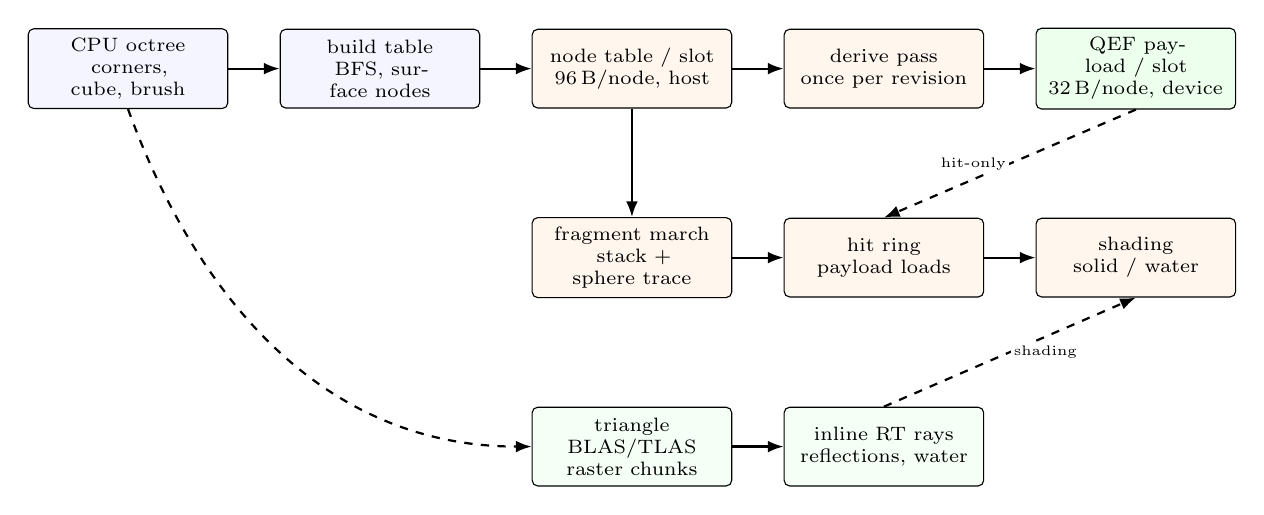
\begin{tikzpicture}[
  box/.style={draw,rounded corners=2pt,align=center,font=\scriptsize,
              minimum height=10mm,text width=23mm,fill=blue!4},
  gpu/.style={box,fill=orange!7},
  pay/.style={box,fill=green!7},
  rt/.style={box,fill=green!4},
  arr/.style={-{Latex[length=2mm]},thick},
  lbl/.style={font=\tiny,fill=white,inner sep=1pt}
]
\node[box] (octree) at (0,0) {CPU octree\\corners, cube, brush};
\node[box] (build) at (3.2,0) {build table\\BFS, surface nodes};
\node[gpu] (table) at (6.4,0) {node table / slot\\96\,B/node, host};
\node[gpu] (derive) at (9.6,0) {derive pass\\once per revision};
\node[pay] (payload) at (12.8,0) {QEF payload / slot\\32\,B/node, device};
\node[gpu] (march) at (6.4,-2.4) {fragment march\\stack + sphere trace};
\node[gpu] (ring) at (9.6,-2.4) {hit ring\\payload loads};
\node[gpu] (shade) at (12.8,-2.4) {shading\\solid / water};
\node[rt] (tlas) at (6.4,-4.8) {triangle BLAS/TLAS\\raster chunks};
\node[rt] (rtrays) at (9.6,-4.8) {inline RT rays\\reflections, water};

\draw[arr] (octree) -- (build);
\draw[arr] (build) -- (table);
\draw[arr] (table) -- (derive);
\draw[arr] (derive) -- (payload);
\draw[arr] (table) -- (march);
\draw[arr] (march) -- (ring);
\draw[arr] (ring) -- (shade);
\draw[arr,dashed] (payload.south) -- node[lbl,left]{hit-only} (ring.north);
\draw[arr,dashed] (octree.south) to[out=-70,in=180] (tlas.west);
\draw[arr] (tlas) -- (rtrays);
\draw[arr,dashed] (rtrays.north) -- node[lbl,right]{shading} (shade.south);
\end{tikzpicture}
\caption{The two scene representations and the derived payload. The SDF
raymarch and the triangle TLAS are independent; the raymarch writes primary
color/depth and the TLAS serves secondary rays. The QEF payload is a sibling
of the node table, not a replacement for any field.}
\label{fig:dataflow}
\end{figure}

\subsection{The CPU octree and its modification model}

An \code{OctreeNode} stores the eight corner samples in \code{float sdf[8]},
the material payload (\code{brushIndex}, \code{textureType}, \code{data},
\code{hsv}), a packed type/flags byte, an LoD byte and a \code{uint version}
(\fpath{space/OctreeNode.hpp:11--33}). Children are stored out of line in a
\code{ChildBlock} of eight node indices
(\fpath{space/ChildBlock.hpp}). The tree is mutated by \code{Octree::apply}
(brush/CSG operations) under a unique lock of \code{treeMutex}; traversals take
a shared lock (\fpath{space/Octree.hpp:35--56}). \code{Octree::shape}
materializes per-node results, including the resolved SDF corner values and
the brush index (\fpath{space/Octree.cpp:891--917}).

Two facts about node versioning are important for cache design:

\begin{itemize}[leftmargin=1.3em,itemsep=1pt]
\item \code{OctreeNode::version} is incremented only for chunk-level surface
      nodes (\fpath{space/Octree.cpp:913--915}) and is not read anywhere else
      in the engine. It is not a usable per-node geometry generation.
      \evS
\item \code{UniqueChangeCollector} explicitly documents that the allocator
      recycles node addresses, so a pointer's version cannot distinguish an
      old and a new occupant of the same address
      (\fpath{space/UniqueChangeCollector.hpp:11--30}). Any cache keyed by a
      CPU node address would therefore be unsound across edits. \evS
\end{itemize}

The only robust generation in the current design is the \emph{whole-table
revision} maintained by \code{MyApp}: \code{raymarchTableVersion_} is incremented
on every rebuild, including an empty result
(\fpath{MyApp.cpp:5220--5223}). Rebuilds are debounced by 0.4\,s
(\fpath{MyApp.cpp:5210--5213}) except after a brush stroke, where the debounce
timer is set past the threshold so the next frame rebuilds
(\fpath{MyApp.cpp:5709--5712}). The revision is a CPU-side \code{uint64_t}; it is
not uploaded to the shader.

\subsection{The GPU node table: 96 bytes}
\label{sec:record}

\code{LocalScene::buildRaymarchTable} walks every enabled Solid and Water layer
breadth-first and appends only \emph{Surface} nodes
(\fpath{utils/LocalScene.cpp:498--718}). Non-surface children are not stored;
their two-bit \code{SpaceType} is packed into the parent's flags, and surface
children dropped by the node cap are marked in a pruned mask and fall back to
the parent's trilinear field. Each record is 96\,B, six \code{vec4}s
(\fpath{utils/OctreeRaymarchTable.hpp:26--39},
\fpath{shaders/includes/octree/RaymarchNodeRecord.glsl:20--40}):

\begin{lstlisting}[language=C++,caption={Shipped GPU node record (96\,B). The child header is a base index plus an 8-bit presence mask.}]
struct RaymarchNode {          // byte offset
    vec4  sdf0;                //   0  corners 0..3
    vec4  sdf1;                //  16  corners 4..7
    vec4  cubeMinSize;         //  32  xyz min, w size
    ivec4 meta;                //  48  x = lod / resolved material,
                               //      y = childBase, z = brush, w = flags
    vec4  hsv0;                //  64  hsv.xyz, textureType
    vec4  hsv1;                //  80  data.xy, 1/Lipschitz, child mask
};
\end{lstlisting}

The child header is compact. The builder appends a parent's stored surface
children consecutively in slot order, so a child resolves from a base index and
a presence mask (\fpath{shaders/includes/octree/RaymarchTable.glsl:58--67},
\fpath{utils/LocalScene.cpp:531, 678}):
\begin{equation}
\code{child}(s)=\code{childBase}+\operatorname{bitCount}\!\bigl(\code{mask}\ \&\ ((1\ll s)-1)\bigr).
\label{eq:child}
\end{equation}
The flags are: bit 0 leaf, bit 1 derived payload valid
(\code{RM_FLAG_PAYLOAD}), bit 2 QEF payload valid (\code{RM_FLAG_QEF}), bits
8--15 pruned surface children, bits 16--31 two-bit child type for non-surface
children (\fpath{RaymarchNodeRecord.glsl:30--40}). The record has no unused
bytes; \code{meta.x} is the LoD in the CPU table and is overwritten by the
resolved material in the derived pass, \code{meta.y} is the child base,
\code{hsv1.z} is the inverse Lipschitz bound and \code{hsv1.w} is the child
mask. \evS

At 96\,B per node the table is 48\,MiB per frame slot; three slots cost
144\,MiB (\fpath{vulkan/renderer/octree/OctreeRaymarchRenderer.hpp:42--50}).
Node and root buffers are created \code{HOST_VISIBLE | HOST_COHERENT},
persistently mapped, and filled with \code{memcpy} on every revision
(\fpath{OctreeRaymarchRenderer.cpp:258--309, 311--339}). A \code{HOST_WRITE ->
FRAGMENT_SHADER} barrier publishes the writes before the solid pass, and the
derive pass adds a \code{HOST_WRITE -> COMPUTE_SHADER} barrier when it runs
(\fpath{OctreeRaymarchRenderer.cpp:370--436}).

\subsection{The derived payload: 32 bytes per node}

The derive pass \fpath{shaders/computation/octree/OctreeDerive.comp} runs one
invocation per stored node, once per table revision per frame slot. It computes
the QEF position, the QEF normal, the resolved material and the Lipschitz bound,
writes the material and inverse bound into the record, and writes the QEF
position/normal into the side buffer
(\fpath{OctreeDerive.comp:52--78}):

\begin{lstlisting}[language=C++,caption={Shipped derive pass. The QEF vectors were already computed for the classifier and are now stored.}]
vec3 qef = sdfCellPosition(sdf, mn, sz);
vec3 n   = sdfCellNormal(sdf, mn, sz, qef);
int  mat = rmResolveMaterialAtCorners(int(nodes[i].meta.z), sdf, mn, sz, qef, n);
float lip = rmLipBound(sdf, sz);

payloads[i].qef    = vec4(qef, 1.0);
payloads[i].normal = vec4(n, 0.0);

nodes[i].meta.x = mat;
nodes[i].hsv1.z = 1.0 / max(lip, 1e-3);
nodes[i].meta.w |= int(RM_FLAG_PAYLOAD | RM_FLAG_QEF);
\end{lstlisting}

The payload entry is two \code{vec4}s, 32\,B, one 32\,B sector per node
(\fpath{utils/OctreeRaymarchTable.hpp:66--73},
\fpath{shaders/includes/octree/RaymarchPayload.glsl:11--15}):

\begin{lstlisting}[language=C++,caption={QEF side payload (32\,B). The \code{w} components are debug tags; \code{qef.w = 1} means written.}]
struct RaymarchPayload {
    vec4 qef;    // xyz = QEF position, w = 1
    vec4 normal; // xyz = QEF normal,   w = 0
};
\end{lstlisting}

The payload buffer is \code{DEVICE_LOCAL}, never mapped by the host, and
allocated lazily with the node buffers
(\fpath{OctreeRaymarchRenderer.cpp:272--281}). If the derive pipeline is
unavailable, a one-entry dummy keeps the descriptor valid and the payload flag
is never set, so the fragment keeps its QEF fallback. The size is
\code{maxNodes * 32} bytes, with \code{maxNodes_} bounded by the device's
storage-buffer range (\fpath{OctreeRaymarchRenderer.cpp:24--25, 275--281}). \evS

\subsection{Roots, upload and revision model}

Each layer contributes a 48\,B root entry: the node index, the stable layer id,
the renderer kind and the layer's conservative surface AABB
(\fpath{utils/OctreeRaymarchTable.hpp:49--60},
\fpath{shaders/includes/octree/RaymarchTable.glsl:28--35}). The AABB is the
union of every stored surface cell cube, plus every pruned surface child's cube;
the layer root cube is deliberately excluded because it spans the whole domain
and would make the test useless. It is only the fallback when the root has no
stored surface child (\fpath{utils/LocalScene.cpp:596--700}). Because a surface
point must lie in a stored surface cell or in a pruned child represented by its
parent, the AABB is conservative. \evS

\code{upload()} copies the table into the slot only when its revision differs
from the slot's recorded revision (\fpath{OctreeRaymarchRenderer.cpp:311--339}).
A new upload marks the slot's \code{needsDerive_} flag; the next recording of
the solid command buffer calls \code{recordDerive()}, which dispatches the
payload pass and publishes its writes before the march
(\fpath{OctreeRaymarchRenderer.cpp:370--436}). A slot that already holds the
revision does nothing. Because the table is rebuilt breadth-first from scratch,
a single edit can renumber every node; node indices are only stable within one
table revision. \evS

\subsection{Ray generation and the root loop}

The pass is a fullscreen triangle (\code{vkCmdDraw(cmd, 3, 1, 0, 0)},
\fpath{OctreeRaymarchRenderer.cpp:490}). The fragment shader reconstructs the
far point with \code{ubo.invViewProjection}, forms
$\vect{r}_o = \code{ubo.viewPosition}$ and
$\vect{r}_d = \mathrm{normalize}(\vect{p}_{far} - \vect{r}_o)$
(\fpath{OctreeRaymarch.frag:1449--1455}). There is no jitter, no MSAA and no
temporal accumulation in this path. \evS

\code{main()} then builds a list of root intervals from each root's rejection
box. The rejection box is the stored-cell surface AABB when tessellation is off,
and the root cube while tessellation displacement is active, because the bump
can move the surface outside the stored cells
(\fpath{OctreeRaymarch.frag:1166--1179}). Roots are inserted in ascending entry
order by a stable insertion sort
(\fpath{OctreeRaymarch.frag:1151--1164, 1470--1479}), marched front to back, and
every later march is clamped to the nearest hit found so far; a root whose entry
is at or behind the hit is skipped entirely
(\fpath{OctreeRaymarch.frag:1481--1495}). Roots past the 16-entry sorting budget
keep the unsorted fallback loop, still with the AABB test and the nearest-hit
clamp (\fpath{OctreeRaymarch.frag:1497--1515}). This is the shipped form of the
first edition's F3. \evS

\subsection{The traversal algorithm}
\label{sec:traversal}

\code{rmMarchRoot} is not a conventional octree DDA. It is a hybrid of
hierarchical descent and sphere tracing inside the current node, closer in
spirit to the PUSH/ADVANCE/POP traversal of Laine and Karras
\cite{laine2010} than to a parametric top-down traversal
\cite{revelles2000}; the octree itself descends from Glassner's space
subdivision \cite{glassner1984}. Its state is a stack of
\code{(nodeId, nodeExit)} pairs, a current node, and the current ray parameter
$t$ (\fpath{OctreeRaymarch.frag:807--1053}). The interval of a ray
$\vect r(t)=\vect r_o+t\vect r_d$ with an axis-aligned cube
$[\vect m,\vect M]$ is computed by the standard slab test
\begin{equation}
a_i=\frac{m_i-r_{o,i}}{r_{d,i}},\qquad
b_i=\frac{M_i-r_{o,i}}{r_{d,i}},\qquad
t_0=\max_i\min(a_i,b_i),\qquad
t_1=\min_i\max(a_i,b_i),
\label{eq:slab}
\end{equation}
with the reciprocals guarded against a zero direction component and hoisted once
per root march (\fpath{OctreeRaymarch.frag:812, 814};
\fpath{RaymarchTable.glsl:130--157}). The child cell is the one containing the
sample point, selected from its local coordinates at a small forward nudge.

\begin{enumerate}[leftmargin=1.4em,itemsep=1pt]
\item \textbf{Root interval.} A slab test computes $[t_0,t_1]$ against the
      root cube; $t \leftarrow \max(t_0,0)$; $t_1$ is clamped to \code{tMax}
      (the nearest hit so far, or infinity); if $t \ge t_1$ the root is
      missed.
\item \textbf{Pop on exit.} If $t \ge \code{nodeExit}$, pop the stack; at depth
      zero the march returns a miss. The root march also returns immediately
      when $t \ge \code{tMax}$.
\item \textbf{Child choice.} If the current node is not a leaf, select the
      child cell containing the sample point at $t+\eta$ ($\eta$ a small
      nudge), and compute the child's exit by a full slab test. If a stored
      Surface child exists, push the current node and descend. If the slot is
      absent and is Empty or Solid, skip to the child's exit without sampling.
      A pruned Surface child (or an exhausted stack) keeps sampling the
      parent's trilinear field up to the child's exit. While tessellation
      displacement is active, the Empty/Solid skip is suspended for displaced
      nodes, because the bump can move the surface across a child border.
\item \textbf{Field sample.} Evaluate the node's trilinear field at
      $\vect{r}_o + \vect{r}_d t$ (plus optional displacement), test
      $|f| \le \epsilon$, and reject a candidate through
      \code{rmHitAllowed} (back-face culling for solids; upward-face test for
      water).
\item \textbf{Sphere step.} Advance by the node's cached
      $|f|/\Lips$ (or $0.5|f|$ when no payload is available), clamped to the
      current child's exit. Sample again at the next point and, on a sign
      change, bisect seven times or refine with the secant when the
      screen-space tolerance is active.
\end{enumerate}

The stack is a fixed \code{RM_MAX_STACK = 16} entries of
\code{(uint,float)}; the step budget is \code{RM_MAX_STEPS = 1024}; the
bisection budget is 7 (\fpath{OctreeRaymarch.frag:135--150}). The source
comment records that grazing rays through the depth-12 lattice can need about
800 steps before reaching the surface
(\fpath{OctreeRaymarch.frag:136--139}). The hit epsilon is
$\max(2\times10^{-3}\,h,10^{-4})$ unless the screen-space tolerance is enabled,
in which case it is widened by the world size of one pixel at the sample
distance (\fpath{OctreeRaymarch.frag:152--164}). \evS

Three properties matter for caching:

\begin{enumerate}[leftmargin=1.4em,itemsep=1pt]
\item \textbf{The ancestor stack is already a traversal cache.} Within one ray,
      the path from the root to the current cell is retained and reused across
      pops. There is no parent pointer in the table and no need for one during
      a march.
\item \textbf{The descent is cheap relative to sampling.} A non-leaf iteration
      adds one child selection and one slab test (about 20 arithmetic
      operations with the reciprocal hoisted) to the sample; a leaf iteration
      adds none. The expensive work is the field evaluation and the hit path.
\item \textbf{The stack is local to \code{rmMarchRoot}.} The hit path does not
      receive it. \code{rmResolveHitShading} and \code{rmBlendAtHit} restart
      from the root for the base point and for every ring quadrant, even though
      the ancestors of the hit node are still in registers when the march
      returns. This is the largest \emph{traversal} redundancy that remains.
\end{enumerate}

\begin{figure}[t]
\centering
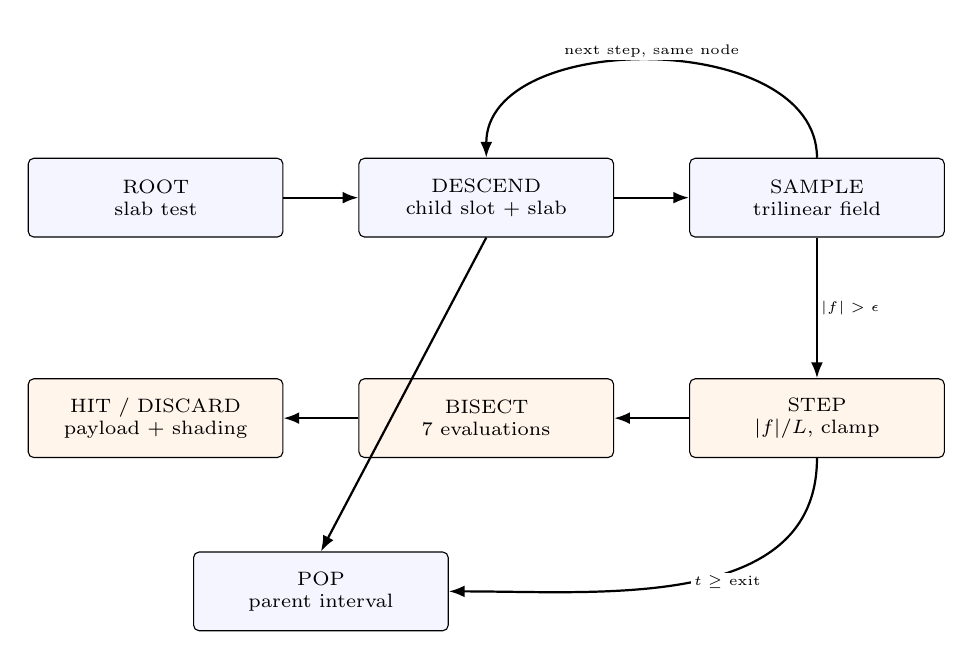
\begin{tikzpicture}[
  st/.style={draw,rounded corners=2pt,align=center,font=\scriptsize,
             minimum height=10mm,text width=30mm,fill=blue!4},
  de/.style={st,fill=orange!8},
  ar/.style={-{Latex[length=2mm]},thick},
  lbl/.style={font=\tiny,fill=white,inner sep=1pt}
]
\node[st] (root) at (0,0) {ROOT\\slab test};
\node[st] (desc) at (4.2,0) {DESCEND\\child slot + slab};
\node[st] (samp) at (8.4,0) {SAMPLE\\trilinear field};
\node[de] (step) at (8.4,-2.8) {STEP\\$|f|/\Lips$, clamp};
\node[de] (bis) at (4.2,-2.8) {BISECT\\7 evaluations};
\node[de] (hit) at (0,-2.8) {HIT / DISCARD\\payload + shading};
\node[st] (pop) at (2.1,-5.0) {POP\\parent interval};

\draw[ar] (root) -- (desc);
\draw[ar] (desc) -- (samp);
\draw[ar] (samp) -- node[lbl,right]{$|f|>\epsilon$} (step);
\draw[ar] (step) -- (bis);
\draw[ar] (bis) -- (hit);
\draw[ar] (step.south) to[out=-90,in=0] node[lbl,right]{$t\ge$ exit} (pop.east);
\draw[ar] (desc.south) -- (pop.north);
\draw[ar] (samp.north) to[out=90,in=90] node[lbl,above]{next step, same node} (desc.north);
\end{tikzpicture}
\caption{The march as a state machine. The stack (not drawn) holds the ancestor
chain and its exit parameters; only one child is descended per sample.
DESCEND$\to$SAMPLE follows a stored surface child; a sign change goes to
BISECT; an Empty/Solid child or a cell exit goes to POP. Empty/Solid children
are skipped by interval, not sampled. The hit path restarts from the root
because the stack is local to \code{rmMarchRoot}.}
\label{fig:state}
\end{figure}

\subsection{SDF evaluation and hit reconstruction}
\label{sec:sdf}

The stored field inside a node is the trilinear reconstruction of the eight
corner samples, renormalized over finite corners when some carry the positive
infinity sentinel (\fpath{RaymarchTable.glsl:102--128}):

\begin{equation}
f(\vect{p}) \;=\; \frac{\sum_{c=0}^{7} w_c(\vect{p})\,d_c}
{\sum_{c=0}^{7} w_c(\vect{p})},
\qquad
w_c = \prod_{a\in\{x,y,z\}} \bigl(1-l_a \text{ if bit}_a(c)=0 \text{ else } l_a\bigr),
\end{equation}
with $\vect{l}=(\vect{p}-\vect{m})/h$ clamped to $[0,1]$. The analytic
trilinear gradient is used for normals
(\fpath{shaders/includes/octree/SdfCell.glsl:70--98}). With tessellation
enabled, a displacement field is folded in as
$f_{\text{bumped}} = f_{\text{base}} - \code{disp}$
(\fpath{OctreeRaymarch.frag:289--297}); with tessellation off (the default,
\fpath{types/Settings.hpp:147}) the displacement is zero and the per-sample
cost is the trilinear evaluation alone. \evS

The per-node material and the step bound are cached in the record. The march's
material lookup is a payload read:
\begin{lstlisting}[language=C++,caption={Material and Lipschitz lookup (simplified from \fpath{OctreeRaymarch.frag:203--221, 996--1004}).}]
int rmResolvedBrush(uint id) {
    if ((uint(rmNodes[id].meta.w) & RM_FLAG_PAYLOAD) != 0u)
        return rmNodes[id].meta.x;          // derive pass result
    int raw = rmNodes[id].meta.z;
    if (raw != LAND_BRUSH_INDEX && raw != NORMAL_BRUSH) return raw;
    return rmResolveMaterialAt(id, rmCellQef(id));   // fallback
}
// step:
float invLip = hasPayload(node) ? rmNodes[node].hsv1.z : 0.5;
stepLen = max(abs(d) * invLip, eps);
\end{lstlisting}

The QEF position and normal are hit-only payload reads:
\begin{lstlisting}[language=C++,caption={QEF and normal lookup (simplified from \fpath{OctreeRaymarch.frag:183--235}).}]
vec3 rmCellQef(uint id) {
    if (rmQefCached(id)) return rmPayload[id].qef.xyz;
    float sdf[8]; for (i) sdf[i] = rmNodeSdf(id, i);
    return sdfCellPosition(sdf, rmNodeMin(id), rmNodeSize(id));
}
vec3 rmNodeNormalAtQef(uint id, vec3 qp) {
    if (rmQefCached(id)) return rmPayload[id].normal.xyz;
    return rmNodeNormal(id, qp);
}
\end{lstlisting}

The expensive per-node QEF/material solve of the first edition is therefore
gone from normal operation. \code{sdfCellPosition} still exists in the fragment
module as the fallback for slots whose derive pass did not run, and
\code{rmResolveMaterialAt} still exists for the same reason. The fallback is a
robustness path, not the hot path. \evS

At a hit, \code{rmHitAllowed} computes the analytic normal at the marched point
to apply back-face culling for solids or the upward-face test for water
(\fpath{OctreeRaymarch.frag:801--805}). \code{rmResolveHitShading} then:
\begin{enumerate}[leftmargin=1.4em,itemsep=1pt]
\item recovers the undisplaced base point when displacement is active; with
      tessellation off, the base point is the hit point and no gradient is
      computed here;
\item descends from the root with \code{rmFindNodeAt} to find the base cell;
\item calls \code{rmBlendAtHit}, which reconstructs the raster path's
      three-material barycentric blend from the four cells around the nearest
      crossing edge. Each probe descends from the root, loads the QEF position,
      loads the material and loads the QEF normal; the fallback solves them
      only when the flags are absent.
\end{enumerate}
So a solid hit currently performs five root descents (base point plus four ring
quadrants), four QEF payload loads, four material loads, four normal loads and
an eight-corner validity test per candidate ring cell. It also computes one
analytic hit-point normal; with displacement active the
water/displacement path can compute up to four (the accepted hit normal, the
base-point normal and up to two fixed-point normals). The ring's QEF arithmetic
is gone; the descents and the blend geometry remain
(\fpath{OctreeRaymarch.frag:482--729, 1066--1117}). \evS

Finally, shading itself is heavy: \code{shadeSolidSurface} evaluates up to
three materials with triplanar mapping, albedo/normal/roughness/AO fetches,
cascaded shadow maps and, in the RT variant, inline reflection rays
(\fpath{shaders/includes/solid/SolidSurface.glsl:86--260}). Any traversal
optimization is bounded by Amdahl's law against this cost. \evS

\subsection{Secondary rays}

There are two secondary-ray paths:

\begin{itemize}[leftmargin=1.3em,itemsep=2pt]
\item \textbf{Hardware RT (preferred when enabled).} The fragment shader
      traces \code{rayQueryEXT} against the triangle TLAS for mirror
      reflections and contact shadows
      (\fpath{shaders/includes/solid/SolidSurface.glsl:272, 457}).
      Water refraction and reflection are resolved through the same TLAS
      (\fpath{RtReflection.glsl:179--300}). The octree is not traversed by
      these rays at all. The engine also has a dedicated half-resolution RT
      water pipeline for the raster path; the octree raymarch does not
      dispatch it.
\item \textbf{SDF water lobes (default when RT shading is off).} A water hit
      calls \code{shadeRaymarchWaterSDF}, which marches the solid roots twice:
      once along the Snell-refracted direction to the lake bed and once along
      the mirror direction; each hit is shaded with \code{shadeSolidSurface}
      (\fpath{OctreeRaymarch.frag:1343--1445}). Both marches build their own
      root interval list and loop every solid root
      (\fpath{OctreeRaymarch.frag:1184--1245, 1381, 1421}).
\end{itemize}

RT shading is selected by \code{settings.rtReflections ||
settings.rtLocalShadows} for the raymarch fragment variant
(\fpath{vulkan/renderer/SceneRenderer.cpp:3140--3144}); the RT water resolve
inside the variant is gated by \code{rt.tlasReady}
(\fpath{OctreeRaymarch.frag:1651--1660}). Both RT toggles default to false
(\fpath{types/Settings.hpp:187, 197}). Thus, in the default configuration, a
water pixel pays for a water-root march, up to five water-ring descents when the
surface is curved, two solid-root list marches (up to four root marches in
total), up to two full solid hit reconstructions (each with five descents) and
up to two \code{shadeSolidSurface} calls. The water fraction of the screen determines
whether this matters. \evS

\subsection{What already is a cache, and what is not}

\begin{center}
\begin{tabularx}{\linewidth}{@{}lX@{}}
\toprule
Existing mechanism & Status for this investigation \\
\midrule
Ancestor stack in \code{rmMarchRoot} & Intra-ray traversal state; already optimal
  for pops. Not reusable across rays without a path. \\
Carry-forward field sample & Intra-ray register reuse of the last sample;
  bit-exact. \\
Material + inverse Lipschitz payload & Once-per-revision record fields; 100\%
  hit rate; invalidated by the table revision. \\
QEF position/normal payload & Once-per-revision device-local side buffer;
  hit-only loads; invalidated by the table revision. \\
Compact child header & Sibling contiguity invariant; base + presence mask. \\
Root surface AABB/order/clamp & Exact per-layer rejection and front-to-back
  scheduling. \\
Whole-table revision & Correct generation for any persistent cache, but not
  currently visible to the shader. \\
Triangle TLAS & The engine's real secondary-ray acceleration structure. \\
Per-frame slots & Three copies of the table and payload for frames in flight;
  not a cache. \\
\bottomrule
\end{tabularx}
\end{center}

There is no per-pixel ray state, no neighbor-shared traversal, no tile cut, no
temporal history, no work queue and no ray sorting. There are also no per-ray
counters in the octree march: the shader contains no atomics and no profile
block. The engine does have a counter precedent in the generic SDF renderer
(\fpath{shaders/renderer/sdf/SdfRenderer.frag:86--96},
\fpath{sdf/types/SdfProfileCounters.hpp}), which this report reuses as the
instrumentation design. \evS

\subsection{The remaining redundancies}
\label{sec:remaining}

The shipped cache removed the QEF/material work, but it did not remove the
following repeated operations. They are listed in descending expected value,
not descending certainty; only the counters of \cref{sec:eval} can settle the
order.

\begin{enumerate}[leftmargin=1.4em,itemsep=2pt]
\item \textbf{Hit-path root descents.} A solid hit performs five
      \code{rmFindNodeAt} descents from the layer root (base point plus four
      ring quadrants). A water pixel can perform up to fifteen (water ring
      plus two solid hits). Each descent repeats the child selection and slab
      test that the march already performed for the hit node's ancestors.
      \evS
\item \textbf{Duplicate accepted-hit normals.} \code{rmHitAllowed} computes
      the analytic normal at the marched point for every candidate. The water
      branch computes the same normal again in \code{main} for the interface
      normal; the displaced-solid branch computes it again in
      \code{rmResolveHitShading}; the ring-fallback branch computes it again if
      the ring did not reconstruct a normal. These are bit-identical calls with
      the same arguments. \evS
\item \textbf{Duplicate reciprocals and root tests.} The caller computes the
      ray reciprocals and tests the root rejection box; \code{rmMarchRoot}
      recomputes the reciprocals and tests the root cube again. The cost is
      three divisions and one box test per root march. \evS
\item \textbf{Bisection with displacement.} Seven field evaluations per hit,
      each with a gradient and up to three texture fetches when displacement is
      active. The screen-space tolerance path already uses a secant refinement;
      the ordinary bisection does not. \evS
\item \textbf{Water secondary shading.} Two full solid hit reconstructions and
      two \code{shadeSolidSurface} calls per water pixel, plus the water
      surface shading. This is the largest absolute per-pixel cost on a
      water-heavy view, but it is a shading/architecture cost, not a reusable
      traversal cache. \evS
\item \textbf{Static QEF fallback footprint.} The QEF solver and the
      material classifier remain in the fragment module as fallbacks. They no
      longer execute in normal operation, but they still influence register
      allocation and instruction-cache footprint. A no-fallback variant is a
      possible experiment. \evS\evP
\item \textbf{Table locality.} The table is breadth-first, so consecutive
      levels are megabytes apart. Siblings are contiguous, but a screen-coherent
      set of pixels at different depths reads widely separated table regions.
      \evS
\item \textbf{Three payload/table copies.} The table and payload are per frame
      slot. Revision sharing would save 96\,MiB of table and 32\,MiB of payload,
      at the cost of a lifetime protocol. \evS
\item \textbf{No counters.} Every estimate in this report is static or
      inherited from the first edition; the engine cannot presently attribute
      time inside the march. \evS
\end{enumerate}

% ============================================================================
\section{Where the time goes now}
\label{sec:bottlenecks}
% ============================================================================

\subsection{A static cost model of one march}

The march's inner loop alternates between two very different cost regimes:
\emph{leaf iterations}, which sample the trilinear field and step, and
\emph{non-leaf iterations}, which additionally select a child and run a slab
test. Table~\ref{tab:cost} lists the operations called by the loop and the
arithmetic they perform. The QEF line is now a fallback; it is included so the
table can be compared with the first edition.

\begin{table}[t]
\centering
\small
\caption{Static cost of the operations in \code{rmMarchRoot} and the hit path,
counted from the source. ``FLOP'' is an approximate multiply/add count;
divisions and square roots are listed separately because their throughput is
much lower on GPUs. These are code-derived estimates, not profiler
measurements. The QEF fallback runs only when the derive payload is absent.}
\label{tab:cost}
\begin{tabularx}{\linewidth}{@{}lXrrr@{}}
\toprule
Operation & Called when & FLOP & div & sqrt \\
\midrule
\code{rmRayBoxInv} (slab test) & every non-leaf iteration; root entry &
  $\approx 20$ & 0 & 0 \\
Child slot selection & every non-leaf iteration & $\approx 10$ & 0 & 0 \\
\code{rmTrilinear} & once per field sample & $\approx 50$ & 1 & 0 \\
\code{rmField} (tess off) & once per field sample & $\approx 55$ & 1 & 0 \\
\code{rmField} (tess on) & adds material lookup and displacement &
  $\approx 10$ & 0 & 0 \\
\code{rmNodeNormal} & per accepted candidate; displaced hit &
  $\approx 50$ & 0 & 1 \\
\code{rmCachedBrush} & per visited node (payload load or fallback) &
  $\approx 5$ & 0 & 0 \\
QEF fallback (source) & only when payload is absent &
  $\approx 940$ & 15 & 20 \\
QEF + normal (compiled) & optimized probe &
  $322$ & 32 & 3 \\
\code{rmFindNodeAt} & per hit/ring descent & $\approx 250$ & 0 & 0 \\
Ring validity test & per candidate ring cell & $\approx 10$ & 0 & 0 \\
Ring payload loads & per ring cell & -- & -- & -- \\
Bisection & on a sign change, 7 iterations & $7\times$ sample & 0 & 0 \\
Secant refinement & only with screen-space tolerance, 2 iterations &
  $2\times$ sample & 0 & 0 \\
\bottomrule
\end{tabularx}
\end{table}

Two conclusions follow directly.

\paragraph{The QEF is no longer in the hot path.} The first edition measured
roughly 62\% of the moderate-terrain march arithmetic as per-node QEF work. In
the current code a visited node reads \code{meta.x} and \code{hsv1.z}; a ring
cell reads 32\,B of QEF payload. The QEF solve executes only when the derive
pass was unavailable. This is a qualitative change, not a marginal one: the
remaining march arithmetic is dominated by trilinear samples, slab tests,
hit-path descents and bisection. \evS\evT

\paragraph{The hit path is now the traversal hotspot.} A solid hit's five root
descents are roughly $5\times12$ child selections and slab tests, about
1\,000--1\,500 arithmetic operations plus node-record loads, before shading.
That is comparable to a long run of march steps. The descents are pure
functions of the hit point and the table, and the march already holds the
ancestor chain; the work is avoidable without any cache memory. \evS\evT

\subsection{Representative ray profiles}

Table~\ref{tab:profiles} builds four synthetic profiles from the source
constants and the reference scene. The numbers are estimates intended to show
proportions, not measured counts. ``Nodes'' counts distinct node entries
(descents and pops); ``iters'' counts march iterations; ``ring'' counts the
root descents performed by the hit path; ``payload'' counts QEF side-buffer
loads. The pre-cache QEF column is the number of solves the first edition would
have performed for the same profile; it is zero in the current normal
operation.

\begin{table}[t]
\centering
\small
\caption{Theoretical per-ray work for four profiles on the reference scene
(two roots, about 30-unit leaves in the first-edition measurements). ``Nodes''
counts distinct node entries; ``iters'' counts march iterations; ``ring''
counts hit-path root descents; ``payload'' counts 32\,B QEF loads. The last
column is the pre-cache QEF solve count, not current work. Estimates only.}
\label{tab:profiles}
\begin{tabular}{@{}lrrrrrr@{}}
\toprule
Profile & roots & nodes & iters & ring & payload & pre-cache QEF \\
\midrule
Sky (upward miss) & 2 & 4 & 16 & 0 & 0 & 0 \\
Terrain (moderate) & 2 & 20 & 120 & 5 & 4 & 24 \\
Grazing terrain & 2 & 60 & 800 & 5 & 4 & 64 \\
Water pixel (RT off) & 5 & 60 & 900 & 15 & 12 & 72 \\
\bottomrule
\end{tabular}
\end{table}

For the moderate terrain profile, the current march arithmetic is roughly
13\,000 FLOP of field/slab/control work plus 1\,200 FLOP of ring descents and
blend geometry. The pre-cache profile added about 22\,000 FLOP of QEF work and
12\,000 FLOP of material-classifier work; the QEF share was the largest single
item. In the current profile the field samples and the hit-path descents are the
largest march items; shading is larger than both. For the grazing profile, the
field work grows to about 88\,000 FLOP, the ring stays near 1\,200, and the
pre-cache QEF work was about 60\,000 FLOP. A scene that mixes simple-brush
cells with LandBrush terrain lowers the old QEF share; the current profile does
not depend on it. With displacement enabled the balance shifts toward texture
fetches, but the QEF remains absent from the ring. \evT

\subsection{Hit-time work}

The per-hit payload is the second concentration of repeated work, now mostly
descents rather than solves. Table~\ref{tab:hitcost} separates a solid hit from
a water pixel.

\begin{table}[t]
\centering
\small
\caption{Estimated per-hit work in the current implementation. ``Descents''
counts \code{rmFindNodeAt} calls from the layer root; ``payload'' counts 32\,B
QEF loads; ``materials'' counts record material loads. The water row assumes a
curved surface (water ring active) and both SDF lobes hitting; flat water skips
the water ring.}
\label{tab:hitcost}
\begin{tabularx}{\linewidth}{@{}lXrrrr@{}}
\toprule
Case & Work & descents & payload & materials & shading \\
\midrule
Solid, tess off & base + 4 ring cells & 5 & 4 & 4 & 1 solid \\
Solid, displaced & base + 4 ring cells + fixed point & 5 & 4 & 4 & 1 solid, extra gradients \\
Water, flat & bed + reflection & 10 & 8 & 8 & 2 solid + water \\
Water, curved & water ring + bed + reflection & 15 & 12 & 12 & 2 solid + water \\
\bottomrule
\end{tabularx}
\end{table}

For a 1280$\times$720 frame every visible terrain pixel pays the solid row once.
Even at one hit per pixel, the five descents are about 1\,000--1\,500 arithmetic
operations plus record loads, comparable to about ten march iterations on the
same pixel. For a water-heavy view the water row can dominate the frame. The
descents are avoidable because the hit node's ancestors are in the march stack;
the shading calls are not avoidable by caching. \evT

\subsection{Cross-layer traversals are now scheduled correctly}

The first edition's clearest duplicate traversal was the root loop: it marched
every root even after a nearer hit and did not clamp later roots. The current
\code{main} fixes that. Roots are sorted by rejection-box entry, a root whose
entry is behind the nearest hit is skipped, and each march stops at
\code{tMax} (\fpath{OctreeRaymarch.frag:1463--1515}). In the reference scene the
water root encloses the opaque root; a terrain hit no longer pays for a complete
water-layer march. The same scheduling is used by the water lobes over the solid
roots (\fpath{OctreeRaymarch.frag:1194--1243}). This is exact and already
shipped. \evS

What remains is not cross-layer duplication but intra-layer hit-path
duplication: the ring and shading restart from the root. That distinction is the
main update from the first edition.

\subsection{Measured pass-level evidence}

The first edition recorded GPU pass timings from a run with the raymarch path
active. The \code{solid} bucket, which hosts the raymarch draw, measured between
141.65\,ms and 505.67\,ms, while depth, sky, water and post-process measured
0.20, 0.11, 1.4--1.7 and 0.26--0.39\,ms respectively. The solid bucket is
roughly two orders of magnitude larger than every other pass. This is strong
evidence that the shaded solid pass dominates the frame in that configuration,
but it does \emph{not} isolate the raymarch: the bucket also contains sky
shading, the fullscreen solid shading and RT work. The run was not a clean A/B,
and the log has since been overwritten. The numbers are cited only as an
order-of-magnitude motivation for instrumentation, not as a speed-up
measurement. \evM

\subsection{Amdahl bounds}

Let $f$ be the fraction of the solid pass spent inside the raymarch traversal
and shading, and $s$ the speed-up applied to that fraction. The overall
solid-pass speed-up is
\begin{equation}
S = \frac{1}{(1-f) + f/s}.
\end{equation}
Table~\ref{tab:amdahl} evaluates this for plausible fractions. Even a perfect
traversal cache (infinite $s$) can only remove $f$. If the march is 40\% of the
solid pass---a reasonable guess given that shading alone fetches nine to fifteen
textures per hit---then eliminating all traversal work yields at most a
1.67$\times$ solid-pass speed-up, and eliminating half of it yields 1.25$\times$.
A change that saves ``only'' the hit-path descents (a few percent of the march)
is invisible at this scale. \evT

\begin{table}[t]
\centering
\small
\caption{Amdahl ceiling for the solid pass. $f$ is the raymarch fraction;
columns are the speed-up at $s=1.25$, $s=1.5$, $s=2$ and $s=\infty$.}
\label{tab:amdahl}
\begin{tabular}{@{}lrrrr@{}}
\toprule
$f$ & $s=1.25$ & $s=1.5$ & $s=2$ & $s=\infty$ \\
\midrule
0.20 & 1.04 & 1.07 & 1.11 & 1.25 \\
0.30 & 1.06 & 1.11 & 1.18 & 1.43 \\
0.40 & 1.09 & 1.15 & 1.25 & 1.67 \\
0.50 & 1.11 & 1.20 & 1.33 & 2.00 \\
0.70 & 1.16 & 1.31 & 1.54 & 3.33 \\
\bottomrule
\end{tabular}
\end{table}

\subsection{Ranked bottlenecks}

The following list orders the remaining inefficiencies by expected value. Items
1--3 are exact, zero-memory changes; items 4--9 are secondary or optional.
None of them is a persistent traversal cache.

\begin{enumerate}[leftmargin=1.5em,itemsep=2pt]
\item \textbf{Hit-path root descents} (\cref{sec:remaining}). Five per solid
      hit, up to fifteen per water pixel. The ancestors are already in the
      march stack; the hit path does not receive them.
\item \textbf{Duplicate accepted-hit normals.} The same analytic gradient is
      solved two or three times for a water hit or a displaced solid hit.
      Pass the accepted normal out of the march.
\item \textbf{Duplicate reciprocals and root tests.} The caller and
      \code{rmMarchRoot} both compute the ray reciprocals and test the root.
      Hoist them into the caller.
\item \textbf{Bisection with displacement.} Seven field evaluations, each with
      a gradient and up to three texture fetches, per hit. A safeguarded secant
      or false-position loop can converge in two or three evaluations.
\item \textbf{Static QEF fallback footprint.} The solver remains in the
      fragment module; a no-fallback variant could reduce register pressure and
      instruction-cache footprint.
\item \textbf{Water secondary shading.} Two full solid hits and two shading
      calls per water pixel. This is the largest absolute cost on a water-heavy
      view, but it is not a traversal cache problem.
\item \textbf{Table and payload locality.} Breadth-first order, 96\,B records
      and three copies. A spatially coherent permutation and revision sharing
      reduce bandwidth and memory, not arithmetic.
\item \textbf{Parametric child selection.} The current child selection
      recomputes local coordinates and a slab test; an incremental DDA-style
      selection saves a few operations per non-leaf iteration.
\item \textbf{No counters.} Every estimate in this section is static; the
      engine cannot presently attribute time inside the march.
\end{enumerate}

% ============================================================================
\section{What can be cached, and when is a cache correct?}
\label{sec:theory}
% ============================================================================

\subsection{A taxonomy}

Five kinds of information could in principle be reused. They have very
different validity conditions and should not be discussed as one thing:

\begin{description}[leftmargin=1.2em,itemsep=2pt]
\item[Derived node payload.] A function of one node's stored corners, cube and
  brush: QEF position, QEF normal, resolved material, Lipschitz bound, maximum
  displacement. Node-constant; invalidated by a table revision; 100\% hit rate;
  no collision. \emph{This is the only persistent cache the current design
  uses.}
\item[Intra-ray state.] The last sample, the current cell exit, the ancestor
  stack, the ray reciprocal, the accepted hit normal. Lives in registers; no
  invalidation; exact.
\item[Inter-ray spatial structure.] A list or cut of nodes shared by a group of
  rays (tile, beam, subgroup). Must cover the group conservatively; otherwise
  it can miss geometry.
\item[Inter-frame history.] Node indices, intervals or hit distances from the
  previous frame. Requires a generation check, a reprojection, and a proof
  that the skipped interval is still empty for the new ray.
\item[SDF values.] Individual $f(\vect{p})$ samples. Sharing requires identical
  or hashed positions; the reuse rate across distinct rays is essentially
  zero.
\end{description}

The current implementation uses the first two. The report rejects the last and
admits the third and fourth only as experiments gated by counters.

\subsection{Validity of a cached starting node}

Suppose a cache returns a node $N$ and an interval start $t_c$ for a ray
$\vect{r}(t)=\vect{r}_o+t\vect{r}_d$. A necessary and sufficient condition for
marching from $N$ to be as correct as marching from the root is
\begin{equation}
\label{eq:valid}
\mathrm{valid}(N,\vect{r},g) =
\underbrace{[g=g_c]}_{\text{generation}}
\land
\underbrace{[\vect{r}\cap\cube(N)\neq\emptyset]}_{\text{containment}}
\land
\underbrace{[t_c\le t_{\text{stop}}]}_{\text{ordering}}
\land
\underbrace{\mathrm{empty}\bigl(\vect{r}[0,t_c]\bigr)}_{\text{prefix}} ,
\end{equation}
where $g$ is the current table revision and $g_c$ the one that produced the
entry. The first three terms are cheap to test. The fourth is the difficult
one: it says that no surface exists between the ray origin and the cached
node's entry. A stored node index and its cube say nothing about the siblings
of its ancestors, and a camera move can put new geometry on the ray's prefix
even when the scene and the table are unchanged. Testing the prefix by
traversal is exactly the work the cache was meant to avoid.

This is the fundamental reason why the naive ``reuse the previous frame's last
node'' design cannot be made exact without either a closed cover (below) or a
full prefix traversal. It can be made \emph{conservative} by only reusing
intervals that a shared structure has already proven empty for the whole group,
which is the tile cut of approach~C. It is also why the \emph{intra-ray}
stack reuse recommended in this edition is different: the stack is not a cached
start node for a new ray, it is the current ray's own ancestor chain, so the
prefix condition is already satisfied by the march that produced the hit.

\subsection{The closed-cover condition}

\begin{definition}
A finite set $\mathcal{S}=\{N_1,\dots,N_k\}$ of octree nodes is a
\emph{closed cut} of a cone $C(T)$ when (i) the cubes cover the cone,
$\bigcup_i \cube(N_i)\supseteq C(T)$; (ii) their interiors are disjoint; and
(iii) each $N_i$ is a node of the current table, or a pruned child represented
by its stored parent \emph{together with the child slot}, so the marched
interval is the pruned child's cube and the overlap condition still holds.
\end{definition}

\begin{theorem}[Closed-cut exactness]
\label{thm:cut}
Let $\mathcal{S}$ be a closed cut for a tile $T$, and let every ray
$\vect{r}\in T$ satisfy $[0,t_{\max}]\subseteq\bigcup_i I_i(\vect{r})$, where
$I_i(\vect{r})$ is the ray interval inside $N_i$. If each node is marched with
the same field, skip rules and epsilon as a full root march, then marching the
nodes in ascending entry order and returning the first hit produces the same
first intersection as a full root march.
\end{theorem}

\begin{proof}[Proof sketch]
The octree cubes partition the root. The cut selects a disjoint subset whose
union covers the ray's interval, so the first surface point along the ray lies
in exactly one $N_i$. Inside $N_i$ the march uses the stored subtree and the
same parent-field fallback as the full march, so it finds the first surface
point in that node. Any node earlier in entry order is surface-free along the
ray, otherwise the first point would lie in it. The minimum over the ordered
nodes is therefore the global first hit.
\end{proof}

The theorem explains both what works and what does not. A tile cut that
conservatively covers the tile's cone is exact. A per-ray cached node is not a
cover: it covers only the node itself, and the prefix is unproven. A
per-subgroup ``shared traversal'' that follows the majority path is not a
cover either: the minority rays may leave the shared path and miss geometry.
An intra-ray ancestor stack is not a cover for a new ray, but it is exact for
the ray that produced it, because the march already visited every ancestor and
the stack records the intervals it traversed.

\begin{figure}[t]
\centering
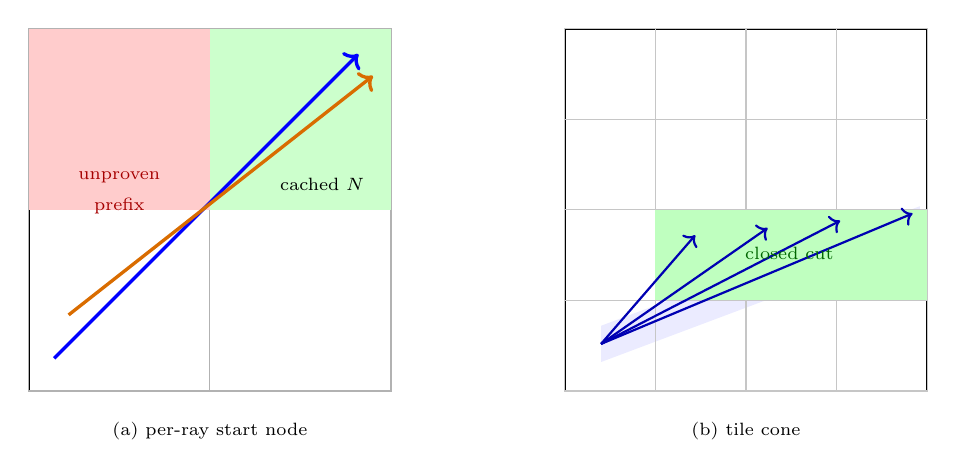
\begin{tikzpicture}[scale=0.92,transform shape]
% left panel: per-ray cached node, invalid prefix
\begin{scope}[xshift=0cm]
  \draw[thick] (0,0) rectangle (5,5);
  \foreach \x in {0,2.5} \foreach \y in {0,2.5}
    \draw[gray!60] (\x,\y) rectangle ++(2.5,2.5);
  \fill[green!20] (2.5,2.5) rectangle (5,5);
  \fill[red!20] (0,2.5) rectangle (2.5,5);
  \draw[->,very thick,blue] (0.35,0.45) -- (4.55,4.65);
  \draw[->,very thick,orange!85!black] (0.55,1.05) -- (4.75,4.35);
  \node[font=\scriptsize] at (4.05,2.85) {cached $N$};
  \node[font=\scriptsize,text=red!65!black] at (1.25,2.95) {unproven};
  \node[font=\scriptsize,text=red!65!black] at (1.25,2.55) {prefix};
  \node[font=\scriptsize] at (2.5,-0.55) {(a) per-ray start node};
\end{scope}
% right panel: tile cone and closed cut
\begin{scope}[xshift=7.4cm]
  \draw[thick] (0,0) rectangle (5,5);
  \fill[blue!8] (0.5,0.4) -- (4.9,2.05) -- (4.9,2.55) -- (0.5,0.9) -- cycle;
  \foreach \x in {0,1.25,2.5,3.75}
    \foreach \y in {0,1.25,2.5,3.75}
      \draw[gray!45] (\x,\y) rectangle ++(1.25,1.25);
  \fill[green!25] (1.25,1.25) rectangle (2.5,2.5);
  \fill[green!25] (2.5,1.25) rectangle (3.75,2.5);
  \fill[green!25] (3.75,1.25) rectangle (5,2.5);
  \foreach \x/\y in {1.8/2.15, 2.8/2.25, 3.8/2.35, 4.8/2.45}
    \draw[->,thick,blue!70!black] (0.5,0.65) -- (\x,\y);
  \node[font=\scriptsize,text=green!40!black] at (3.1,1.9) {closed cut};
  \node[font=\scriptsize] at (2.5,-0.55) {(b) tile cone};
\end{scope}
\end{tikzpicture}
\caption{Why the cover condition is necessary. (a) A node cached from a
previous ray (blue) only proves the node itself empty/non-empty; the current
ray (orange) has an unproven prefix in a different sibling. (b) A cut generated
from the tile's conservative cone covers every ray's interval and can be
validated per node with box tests.}
\label{fig:cut}
\end{figure}

\subsection{Generation and invalidation}

The only current generation that is safe for persistent caches is the
whole-table revision (\fpath{MyApp.cpp:5220--5223}). It has three useful
properties: it changes on every rebuild, it changes even when the rebuild
produces an empty table, and it is cheap to compare. It has one drawback: it
is not uploaded. The push constant has three unused words
(\fpath{OctreeRaymarchRenderer.hpp:56--64}), so exposing the revision costs
nothing and should be done before any persistent cache is added.

Per-node versions are \emph{not} usable today. \code{OctreeNode::version} is
incremented only for chunk nodes and never read
(\fpath{space/Octree.cpp:913--915}); the allocator recycles node memory, so
address-keyed version checks are unsound
(\fpath{space/UniqueChangeCollector.hpp:11--30}). If partial table updates
are ever introduced, a GPU-side per-node generation must be added and bumped
by the builder, not by the node.

The QEF side payload has a different validity model: it is written by the
derive pass for every node of the revision, in the same slot, before the march.
The fragment checks \code{RM_FLAG_QEF} before reading it, so an unrun or failed
derive pass falls back to the solver. No revision word is needed for this
payload because the slot's table and payload are produced together and the slot
is fenced before the host rewrites it. A future revision-shared payload would
need the revision or a generation flag in the buffer.

\subsection{Coherence arithmetic for this camera and this scene}

The horizontal angular size of one pixel is
\begin{equation}
\Delta\theta_{\text{px}} = \frac{2\tan(\theta_{\text{fov}}/2)}{W}.
\end{equation}
At a 60$^\circ$ horizontal field of view and $W=1280$,
$\Delta\theta_{\text{px}}\approx 9.0\times 10^{-4}$\,rad
($\approx 0.052^\circ$). A tile of $n\times n$ pixels subtends
$n\Delta\theta_{\text{px}}$ and covers a world footprint of about
$z\,n\,\Delta\theta_{\text{px}}$ at distance $z$. With 30-unit leaves (the
first-edition reference measurement), an 8$\times$8 tile's footprint equals one
leaf only at $z\approx 4157$\,m; a 4$\times$4 tile at $z\approx 8314$\,m; a
16$\times$16 tile at $z\approx 2078$\,m. Inside the 15.36\,km terrain, all
these tiles are usually smaller than a leaf cell in object space. Neighboring
rays really do visit the same nodes. The benefit is bounded because the
agreement is in the cheap part of the march, while the expensive per-sample
work and shading remain per-ray. The current leaf size is scene-dependent; use
the scene's actual cell size when applying this arithmetic. \evT

Temporal coherence is much weaker. A camera rotation of $\omega$ degrees per
second shifts the image by
\begin{equation}
\Delta p = \frac{\omega}{f_{\text{fps}}\,\Delta\theta_{\text{px}}}
\end{equation}
pixels per frame. At 60\,fps and 1280 pixels this is 0.322 pixels per
degree/second; a 90$^\circ$/s turn moves the image 29 pixels in one frame.
Even at 30\,fps a 10$^\circ$/s pan moves it 6.4 pixels. A per-pixel temporal
cache is therefore only valid for near-static cameras (below about
3.1$^\circ$/s at 60\,fps for a one-pixel budget). Translation adds disparity:
$\Delta p\approx f_{\text{px}}\,b/z$ for a baseline $b$ at depth $z$, with
$f_{\text{px}}=W/(2\tan(\theta_{\text{fov}}/2))\approx 1108$ at 1280/60$^\circ$;
a 1\,m strafe at 100\,m is 11 pixels. Figure~\ref{fig:temporal} plots the
rotation case. \evT

\begin{figure}[t]
\centering
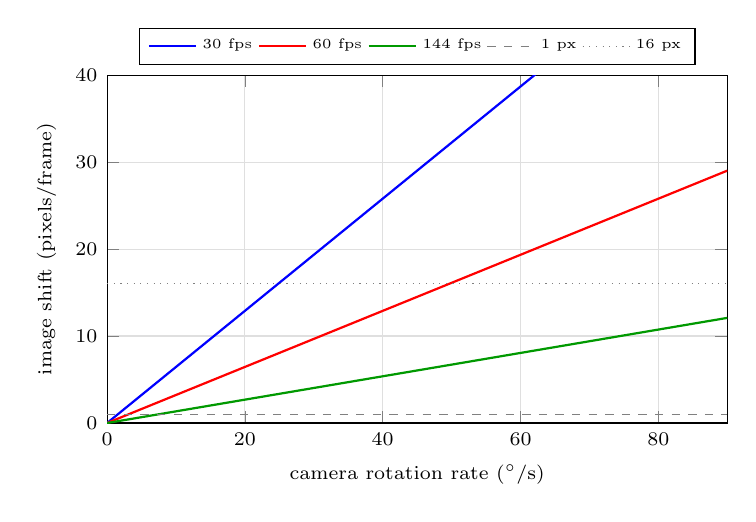
\begin{tikzpicture}
\begin{axis}[
  width=0.78\linewidth,height=6.0cm,
  xlabel={camera rotation rate ($^\circ$/s)}, ylabel={image shift (pixels/frame)},
  xmin=0,xmax=90,ymin=0,ymax=40,
  grid=major,grid style={gray!25},
  tick label style={font=\scriptsize},label style={font=\scriptsize},
  legend style={font=\tiny,at={(0.5,1.03)},anchor=south,legend columns=5},
]
\addplot[thick,blue,domain=0:90,samples=2]{0.6449*x};
\addplot[thick,red,domain=0:90,samples=2]{0.3224*x};
\addplot[thick,green!60!black,domain=0:90,samples=2]{0.1343*x};
\addplot[dashed,gray,domain=0:90,samples=2]{1};
\addplot[dotted,gray,domain=0:90,samples=2]{16};
\legend{30 fps, 60 fps, 144 fps, 1 px, 16 px}
\end{axis}
\end{tikzpicture}
\caption{Per-frame image shift caused by camera rotation, at 1280 pixels and a
60$^\circ$ horizontal FOV. A same-pixel history is only valid below the 1-pixel
line; a 16$\times$16 tile tolerates about 0.83$^\circ$/frame, i.e.\ 50$^\circ$/s
at 60\,fps, and even then its rays see different geometry.}
\label{fig:temporal}
\end{figure}

\subsection{Cost--benefit model for a cache}

For a cache with hit rate $h$, validation cost $V$, hit cost $C_h$ and miss
cost $C_m$, the expected cost is
\begin{equation}
C = V + h\,C_h + (1-h)\,C_m ,
\end{equation}
to be compared with the baseline $C_b$. A cache is worthwhile only when
$C<C_b$ \emph{and} its validation is exact. For the node payload cache,
$h=1$, $V=0$ (the flag check is one test per access) and $C_h$ is a load; this
is the best possible position. For a temporal start node, $h$ is set by the
motion in Figure~\ref{fig:temporal}, $V$ includes a reprojection and a
generation check, and the prefix proof is still missing; the expected value is
negative or, at best, a few percent. For the intra-ray stack reuse, $h$ is 1
for the ray that produced the stack, $V$ is a containment test per level, and
the fallback is the current root descent, so the design is exact by
construction.

\subsection{Memory budget}

Table~\ref{tab:memory} lists the candidates and their footprint at the
reference cap of 524\,288 nodes and 1280$\times$720. The table and payload are
already 64\,MiB per slot; the remaining candidates are either free or rejected.
Temporal and tile candidates are cheap in isolation but buy little; a global
value cache is both large and useless.

\begin{table}[t]
\centering
\small
\caption{Memory budget of the cache candidates at 524\,288 nodes, three
frames in flight, 1280$\times$720 (921\,600 pixels). ``Per slot'' is the
allocation actually touched by one frame; totals assume three slots unless the
entry is revision-shared.}
\label{tab:memory}
\begin{tabularx}{\linewidth}{@{}lrrX@{}}
\toprule
Candidate & per slot & total & Notes \\
\midrule
Current node table (96\,B) & 48.0\,MiB & 144.0\,MiB & host-visible \\
Current QEF payload (32\,B) & 16.0\,MiB & 48.0\,MiB & device-local, hit-only \\
Root entries (256 $\times$ 48\,B) & 12\,KiB & 36\,KiB & host-visible \\
Revision-shared table & 48.0\,MiB & 48.0\,MiB & saves 96\,MiB; lifetime protocol \\
Revision-shared payload & 16.0\,MiB & 16.0\,MiB & saves 32\,MiB; lifetime protocol \\
In-record QEF (128\,B record) & 64.0\,MiB & 192.0\,MiB & +33\% traversal traffic; rejected \\
Tile cut (16$\times$16, 8 nodes) & 0.23\,MiB & 0.69\,MiB & rejected; expected net loss \\
Temporal history (16\,B/pixel) & 14.7\,MiB & 44.2\,MiB & rejected; low hit rate \\
Global SDF value hash (4M) & 64.0\,MiB & 64.0\,MiB & rejected; near-zero reuse \\
\bottomrule
\end{tabularx}
\end{table}

The shipped table+payload footprint is exactly 192\,MiB across three slots,
the same as the old 128\,B record alone. The difference is that the traversal
stride is 96\,B and the extra 32\,B is paid only at hits. This is the central
storage result of \fpath{qef_gpu.tex}, and it remains valid.

% ============================================================================
\section{Approach analysis}
\label{sec:approaches}
% ============================================================================

This section evaluates each requested approach against the implementation
described in \cref{sec:existing}. The comparison table at the end of the
section summarises the verdicts; \cref{sec:ranking} ranks what remains.

\subsection{A. Per-ray traversal caching}
\label{sec:A}

\paragraph{What already exists.} Within a single ray, the ancestor stack is a
traversal cache: a pop restores the parent and its exit interval without
re-descending. The carry-forward sample reuses the last field value. The stack
is exact by construction and costs no memory beyond the invocation. Any
proposal in this category must beat that, not the naive ``start from the root
at every step'' straw man.

\paragraph{A1: reuse the last node as the next starting point.} Already done.
When the ray stays inside a node, the loop reuses the node's field and material
cache; when it leaves, it pops to the parent and descends into the next child.
There is no redundant descent in the current loop. \evS

\paragraph{A2: a persistent per-ray start node across frames.} The obvious
design stores, per pixel, the node that contained the previous frame's hit and
starts the next frame's march there. It fails the prefix condition in
\cref{eq:valid}. Even with an unchanged table and a static camera, the new ray
may pass through geometry that the old ray did not; with a moving camera this
happens routinely. Validating the prefix is a traversal of the skipped
interval, which removes the benefit. A \emph{conservative} variant is possible
only when the skipped interval is covered by a structure that has been proven
empty for the whole pixel group (approach~C) or when the cache stores a
previously computed \emph{empty interval} for the same ray direction (which
camera motion invalidates). The safe fallback is a full root march, which
makes the cache a hint rather than an optimization.

\paragraph{A3: a persistent per-ray stack.} Storing the previous frame's stack
and validating each level against the new ray is cheap per level (one box
test), but the validation of $d$ levels costs about as much as descending them
in the first place: the descent is one child selection and one slab test per
level. The only saving would be the node-record loads, which the L1 cache
already provides for a coherent neighborhood. The expected gain is below the
noise floor of the shading cost.

\paragraph{A4: intra-ray hit-stack reuse.} This is the useful form and is
\emph{not} a persistent cache. The march already holds the ancestor chain of
the hit node. If the stack and its depth are made visible to
\code{rmResolveHitShading} and \code{rmBlendAtHit}, the base-point and ring
descents can start from the deepest ancestor whose cube contains the query
point instead of from the root. The descent decisions depend only on the query
point, so starting from a containing ancestor is exact; if no ancestor
contains it, fall back to the root. This removes up to five root descents per
solid hit and up to fifteen per water pixel with zero extra memory. It is the
top recommendation of this edition (\cref{sec:rec}). \evP

\paragraph{Invalidation and divergence.} Node indices are only valid within a
table revision, so any persistent entry needs the revision (currently not
exposed to the shader). Rays that diverge from the cached path must drop the
invalid suffix and re-descend; a path prefix that is valid for the origin but
not for the direction is the common case at silhouettes. The bookkeeping
(validate, truncate, fall back) is more expensive than the saved descent. The
intra-ray stack has no invalidation problem: it belongs to the invocation that
produced it.

\paragraph{Verdict.} A1 and A4 are already implemented or recommended; A2/A3
are not exact without a closed cover and have a theoretical ceiling of a few
percent. \textbf{Do not build persistent per-ray caches.} If a temporal
experiment is desired later, restrict it to a \emph{hint} that reorders work,
never to a skip of unvalidated space, and gate it behind the counters of
\cref{sec:eval}.

\subsection{B. Neighboring-ray traversal sharing}
\label{sec:B}

\paragraph{What could be shared.} Adjacent primary rays have nearly identical
directions and origins, so they visit the same octree nodes for most of the
path. The coherence arithmetic in \cref{sec:theory} shows that an 8$\times$8
tile's world footprint is smaller than a 30-unit leaf out to about 4.2\,km.
The agreement is therefore high in object space---higher than one might expect
from a generic BVH scene. The question is not whether the rays agree, but
whether exploiting the agreement is cheaper than independent traversal on this
GPU.

\paragraph{B1: 2$\times$2 fragment quads.} A fragment shader's only group with
guaranteed 2$\times$2 pixel adjacency is the quad. All four lanes could compute
the child slot at each level, ballot on agreement, and have one lane broadcast
the child index and the node record. The other lanes then sample their own
field values. The saving is three quarters of the descent arithmetic and node
loads for the shared prefix; the per-ray sampling, stepping and bisection
remain. Packet traversal is the classic coherence strategy on CPUs
\cite{wald2001}, but on GPUs the measurement below favors independent
traversal. Because the descent is a small fraction of the march
(\cref{tab:profiles}), the ceiling is low. The cost is a ballot, a broadcast
and a branch per level, plus handling helper invocations and quad lanes that
have terminated. \evT

\paragraph{B2: 4$\times$4 and 8$\times$8 shared traversal.} These groups are
larger than a quad and cannot be formed portably in a fragment shader without
shared memory and workgroup cooperation, which fragments do not have. They
would require a compute prepass or a workgroup-based renderer. A compute
prepass that builds a per-tile cut is approach~C; a shared depth-first
traversal inside a compute workgroup is a different architecture (see F8).
In both variants the sharing covers only \emph{traversal}; each ray still
evaluates its own trilinear field, steps and bisection. That is the expensive
part, which is why a shared candidate-node list or a shared traversal followed
by independent per-ray SDF evaluation has a limited payoff here.

\paragraph{B3: beams and conservative frustums.} The best-known form is the
beam optimization of Laine and Karras \cite{laine2010}: cast a coarse pass for
the corners of a 4$\times$4 or 8$\times$8 block, terminate the coarse traversal
when the visited voxel is no longer large enough to cover at least one ray of
the block, and start each fine ray at a conservative distance derived from the
coarse result. The key is that the coarse pass stops descending once the voxel
is smaller than the beam, so a sub-voxel feature cannot hide. \evR

Adapting this to an SDF octree is possible in principle: the coarse pass would
use the node's trilinear field and stop at the depth where the node's screen
footprint falls below one pixel. The output would be a conservative starting
distance per tile, not a node. It would skip the empty prefix, not the
near-surface march, and the empty prefix is already skipped cheaply by the
Empty/Solid child intervals. The expected gain is again small. \evT

\paragraph{Why GPUs often prefer independent traversal.} Aila and Laine
measured packet traversal (all rays in a warp share the traversal stack) and
per-ray traversal on a GTX 285. Packet traversal was a factor 1.7--2.4 below
the simulated optimum even for coherent primary rays, while per-ray traversal
was faster than packet traversal in every tested ray class; the gap was not
explained by memory bandwidth \cite{aila2009}. The engine's fragment shader is
already a per-ray traversal with hardware-managed quads, which is the
configuration that paper found preferable. \evR

\paragraph{Verdict.} High implementation complexity (ballots, helper
invocations, divergence, fallback), low ceiling (descent share), and a
literature that does not support packet sharing on GPUs for this ray class.
\textbf{Do not build as a first step.} A 2$\times$2 ballot experiment is
defensible only after instrumentation shows the descent is more than 15\% of
the march.

\subsection{C. Screen-space tile traversal caching}
\label{sec:C}

\paragraph{Design.} A compute prepass divides the screen into $n\times n$
tiles, traverses the octree once per tile with a conservative cone/frustum,
and writes a compact list of nodes forming a closed cut (a traversal frontier,
in the octree sense). Each entry stores the node index and its entry/exit
parameters along the tile's center ray, plus a revision tag. The fragment
shader reads its tile's list, box-tests the entries, and marches the first
entry whose interval contains the ray.

\paragraph{Exactness.} The design is exact if the cut covers the whole cone and
the ray interval, as proved in Theorem~\ref{thm:cut}. Two details are easy to
get wrong: the cut must cover the cone for \emph{all} rays in the tile (not
just the center ray), and it must cover the entire ray interval, including the
part behind the first surface (otherwise a ray that misses the first node can
fall off the end of the list). The second requirement forces either a
full-volume cut (many nodes) or a fallback to the root march after the last
entry, which reintroduces the descent.

\paragraph{Cost.} At 1280$\times$720 and 16$\times$16 tiles there are 3600
tiles. Even at 1000 node tests per tile the prepass is 3.6M tests, versus
roughly 46--184M node tests for 921K rays at 50--200 visits each: 2--8\%
additional work. The saving per ray is the initial descent, one to three
percent of the march. The prepass therefore costs more than it saves. An
8$\times$8 tile doubles the prepass; a 32$\times$32 tile reduces the prepass but
makes the cut wider and the per-ray list walk longer. A per-frame prepass also
adds a compute-to-fragment dependency before the solid pass: the whole prepass
must finish before the first pixel marches. The payload pass has the same
barrier but runs once per revision, not once per frame. \evT

\paragraph{The list-walk problem.} A cut of $k$ entries requires up to $k$ box
tests per ray to find the entry containing the ray. A descent to depth 12 also
requires about 12 box tests. Unless $k\ll 12$, the list walk is not cheaper
than the descent it replaces. For a cone that covers the full ray interval,
$k$ is typically larger than 12.

\paragraph{Per-tile ancestor chain.} A cheaper variant stores the ancestor
chain of a representative surface node (about 10 nodes) and pre-fills the
march's stack. The fragment must validate each ancestor's cube against its own
ray (10 box tests) and re-derive the child slots (10 selections); that is the
same work as descending. The saving cancels. \evT

\paragraph{Verdict.} Theoretically exact only as a closed cut, practically a
net loss because the descent is cheap and the cut must be wide. \textbf{Do not
build} unless counters show the descent is a large fraction of the march (they
will not, given \cref{tab:profiles}). If a tile prepass is ever built for
another purpose (e.g.\ occlusion culling), the cut can be a by-product, but it
should not be the reason.

\subsection{D. Secondary-ray traversal caching}
\label{sec:D}

\paragraph{Two worlds.} When hardware RT is enabled, secondary rays traverse
the triangle TLAS; the octree is not involved
(\fpath{RtReflection.glsl:179--300}). When RT shading is off (the default,
\fpath{types/Settings.hpp:187, 197}), a water hit marches the solid roots
twice in the same shader (\fpath{OctreeRaymarch.frag:1343--1445}). Any octree
secondary cache is therefore only relevant to the second configuration, and
only to water pixels. The water fraction of the frame is scene-dependent and
must be measured. Secondary rays from neighboring water pixels are themselves
coherent---the lake surface is smooth---but the TLAS already exploits that
coherence with a hardware-traversed BVH. An SDF-side secondary index would
have to match it before it could help.

\paragraph{D1: reuse the primary solid path for the refracted ray.} The first
edition proposed passing the primary solid stack to the refraction march. That
design is no longer applicable: the primary root loop sorts and clamps roots,
so a water hit stops the solid root march at the water distance. The primary
ray does not reach the lake bed; there is no solid stack to pass. The
refraction march is a genuinely new ray with a different origin and direction.
The only shared data are the layer AABBs and the node table, which the march
already uses. \evS

\paragraph{D2: reuse the water node for the reflection ray.} The reflection
origin is the wave-displaced water point. The water node's cube contains it,
but the reflection direction points away from the water body, and the water
node's subtree is small. The cached node is valid for a short interval only;
beyond it, there is no parent link to continue. Not worth it.

\paragraph{D3: separate caches per ray type.} Reflection and refraction have
different origins and directions; a shared cache would thrash. Separate caches
would double the memory and still have low hit rates because the origins vary
per pixel. Reject.

\paragraph{D4: a spatial index for secondary rays.} The triangle TLAS already
is that index. Building an SDF-side index would duplicate it and would not
cover the rasterized objects (vegetation, props) that the TLAS covers. Reject.

\paragraph{Verdict.} Keep the TLAS for secondary visibility. The SDF water
lobes are shading-bound, not traversal-bound; improving them is a rendering
architecture question (half-resolution, RT fallback, denoising), not a cache
question. \textbf{No separate secondary cache.}

\subsection{E. Temporal traversal caching}
\label{sec:E}

\paragraph{What would be stored.} Per-pixel previous-frame start nodes,
previous hit distances, or previous stacks. The cache key would be the pixel
(or a reprojected position), the value a node index or interval, and the
validity a generation plus a reprojection plus a prefix proof.

\paragraph{Why it is weak here.} The engine has no temporal history
infrastructure for the raymarch: no jitter, no velocity buffer, no TAA, and no
previous-frame matrices in the non-RT scene UBO. \code{rt.prevViewProj} exists
only in the RT parameter block (\fpath{vulkan/renderer/rt/RayTracingParams.hpp:16},
binding 17 in \fpath{RtSceneBindings.glsl:22--25}), so the non-RT raymarch
cannot reproject without new plumbing. The arithmetic in
Figure~\ref{fig:temporal} shows that a same-pixel history survives only
near-static cameras; a neighborhood search would be needed for normal play,
which is a full TAA-style subsystem. Even with perfect reprojection, the prefix
is unproven (approach~A), and the generation changes on every brush stroke.
Reprojection with a color/depth history is the standard temporal technique in
games \cite{pedersen2016}; the engine has no such history for the raymarch.

\paragraph{Hit-distance hints.} A cheaper temporal signal is the previous
frame's hit distance, used to cap the march or to choose a step budget. It is
approximate: a hill can enter the ray path, and there is no temporal
antialiasing to hide the resulting popping. It also does not help the
expensive near-surface grazing steps, which are where the time goes. Reject
unless a temporal filter is added for other reasons.

\paragraph{Temporal reuse of secondary rays.} Secondary reuse is weaker still.
The water surface is animated by the wind field: \code{sky.windTime} advances
every frame (\fpath{OctreeRaymarch.frag:1267--1268}), so the wave normal and the
reflection/refraction directions change even with a static camera. A per-pixel
history of a secondary origin or direction is therefore stale for reasons
unrelated to camera motion.

\paragraph{Verdict.} \textbf{Do not build now.} Revisit only if the engine gains
a reprojection/TAA infrastructure; then a per-tile (not per-pixel) traversal
history is the only form with enough rays to amortize validation.

\subsection{F. Alternative approaches}
\label{sec:F}

\paragraph{F1: carry-forward of the last sample.} Shipped. The loop evaluates
the field at $t$ and at $t+\Delta t$, then reuses the second value when the next
iteration has the same node and $t$
(\fpath{OctreeRaymarch.frag:826--835, 943--950, 1041--1050}). The reuse
condition is exact, so the common leaf case performs one field evaluation per
iteration instead of two. \evS

\paragraph{F2: node payload cache.} Shipped in two layers. The derive pass
writes the resolved material into \code{meta.x} and the inverse Lipschitz bound
into \code{hsv1.z} (\code{RM_FLAG_PAYLOAD}); the QEF position and normal go to
the 32\,B side buffer (\code{RM_FLAG_QEF}). The march reads the material and
step bound per visited node; the hit ring reads the QEF vectors per ring cell.
The maximum displacement is not cached per node; it is derived from the
material at each displaced sample. \evS

\paragraph{F3: root-level reuse.} Shipped. Each root stores a conservative
surface AABB; roots are sorted by entry, rejected when missed, and every march
is clamped to the nearest hit so far
(\fpath{OctreeRaymarch.frag:1166--1179, 1470--1515}). While tessellation
displacement is active, the rejection box falls back to the root cube so the
bump cannot escape the box. \evS

\paragraph{F4: compact traversal header.} Shipped. The record is 96\,B with a
child base plus an 8-bit presence mask; slot $s$ resolves by
\cref{eq:child}. The child contiguity invariant is established by the
builder's append order and documented in the shared header; a CPU-side
assertion that the stored children are contiguous is still recommended as a
debug check. \evS

\paragraph{F5: parametric child selection (DDA).} Not shipped. The current loop
recomputes the child slot with \code{floor(local*2)} and a full slab test every
non-leaf iteration. A parametric octree traversal \cite{revelles2000} computes
the three splitting-plane parameters incrementally and selects the child by
comparisons, avoiding most of the slab arithmetic; the same incremental idea
underlies the grid DDA of Amanatides and Woo \cite{amanatides1987}. The
engine's surface-node-only table and pruned fallback complicate a pure DDA,
but the child-selection part is replaceable. Expected gain is a few percent;
complexity is moderate. \evP

\paragraph{F6: stackless traversal.} Rejected. A bitmask-based stackless
traversal reduces per-ray state from hundreds of bytes to about 12\,B
\cite{afra2014}. However, the same paper measured stackless traversal as
20--31\% \emph{slower} on a GPU for ordinary ray tracing; its advantage is the
number of rays in flight, not speed per ray. The engine's stack is now 16
entries (128\,B), which matches the measured maximum depth 12, so the state
saving is already captured without changing the algorithm. A full stackless
rewrite is not justified. \evP

\paragraph{F7: ray sorting and packets.} Rejected. Sorting rays into coherent
packets and traversing a frustum breadth-first gave a $3\times$ speed-up over a
depth-first tracer in Garanzha and Loop \cite{garanzha2010}, but the technique
targets incoherent secondary rays, requires a multi-stage compute pipeline
with scans and compaction, and shuffles rays away from the raster/depth order
that the engine depends on for \code{gl_FragDepth}. Primary rays in a
rasterizer are already coherent, so sorting adds cost without adding
coherence. \evR

\paragraph{F8: wavefront and work queues.} Rejected. Persistent-thread work
queues can recover 1.5--2.2$\times$ for packet traversal in Aila and Laine
\cite{aila2009}, mainly by improving work distribution for heterogeneous rays.
The engine's primary march is a fragment pass with inline ray queries and
depth writes; moving it to a compute wavefront would require a G-buffer, a
deferred shading pass, and a replacement for the inline RT calls, i.e.\ a new
renderer. It also contradicts the instruction to preserve the Vulkan
architecture. \evR

\paragraph{F9: SVO/DAG representations.} Rejected. Sparse voxel octrees and
DAGs \cite{laine2010,garanzha2010} replace the representation and store
occupancy and contours, not eight SDF corners. The task explicitly forbids
replacing the octree representation. More importantly, the SDF march needs the
corner values for interpolation and QEF, which a voxel occupancy DAG does not
carry.

\paragraph{F10: hierarchical traversal caches.} Covered by the closed cut of
approach~C. A hierarchy of cached cuts (one per depth) adds memory and
validation without changing the conclusion.

\paragraph{F11: screen-space hit epsilon and refinement.} Shipped, opt-in,
default off. The current \code{rmHitEpsilon} widens the world-space floor by the
world size of one pixel at the sample distance when
\code{ubo.raymarchScreenEps > 0}; the accepted hit is refined by a two-step
secant clamped to the band (\fpath{OctreeRaymarch.frag:152--164, 299--323}).
The setting default is 0 (\fpath{types/Settings.hpp:158--161}). The remaining
work is validation and a decision to enable it, not implementation.
\evS\evP

\paragraph{F12: SDF value caches.} Rejected; see \cref{sec:sdfcache}.

\paragraph{F13: hit-stack reuse.} Recommended. Pass the march's ancestor stack
and depth to the hit path; start \code{rmFindNodeAt} from the deepest ancestor
whose cube contains the query point, with a root fallback. Exact, zero memory,
and removes up to five descents per solid hit. See \cref{sec:rec}.

\paragraph{F14: accepted-normal reuse.} Recommended. Return the analytic normal
computed by \code{rmHitAllowed} with the hit, and use it in the water branch,
the displacement fixed point, and the ring fallback. The call arguments are
identical, so the result is bit-identical; the change removes one gradient per
water or displaced hit. See \cref{sec:rec}.

\paragraph{F15: reciprocal and root-interval hoist.} Recommended. The caller
already computes the ray reciprocals and a rejection-box interval; pass them
into \code{rmMarchRoot} instead of recomputing them. Exact, small.

\paragraph{F16: no-fallback fragment variant.} Optional. The QEF solver and
classifier remain in the fragment module for robustness, even when the derive
pass is guaranteed. A separate module or a specialization constant that
compiles the fallback out could reduce register pressure and instruction-cache
footprint. The trade is an extra pipeline variant and a stricter precondition
(derive must succeed); measure before shipping. \evP

\paragraph{F17: max displacement in the payload.} Optional. The payload's
\code{normal.w} is reserved and zero; it could hold the node's maximum
displacement magnitude for tessellation-on paths, replacing a per-sample
material lookup. This only matters when tessellation is enabled (off by
default) and does not change the QEF cache. \evP

\paragraph{F18: revision-shared table/payload.} Optional memory optimization.
The table and payload are copied per frame slot; one immutable revision shared
by all slots would save 96\,MiB (table) and 32\,MiB (payload), at the cost of a
lifetime protocol and descriptor updates after the slot fence. This is a
memory/bandwidth change, not an arithmetic one. \evP

\subsection{Comparison table}

\begin{table}[t]
\centering
\scriptsize
\setlength{\tabcolsep}{3pt}
\caption{Approaches against the current implementation. ``Gross gain'' is
relative to the raymarch time, not the frame, and is a theoretical estimate
from the static cost model unless marked. ``Mem'' is incremental. Rows marked
``shipped'' are not candidates; they are included so the table can be compared
with the first edition.}
\label{tab:approaches}
\begin{tabularx}{\linewidth}{@{}p{3.3cm}p{3.2cm}p{1.6cm}p{1.5cm}p{2.2cm}p{2.2cm}@{}}
\toprule
Approach & Mechanism & Mem & Gross gain & Complexity/risk & Verdict \\
\midrule
A per-ray history & prev node/stack & 8--160\,B & 1--4\% & high/high & reject \\
A4 hit-stack reuse & pass march stack & 0 & 3--10\% & low/very low & \textbf{do} \\
B neighbour sharing & 2$\times$2, 4/8$\times$8, beams & 0--4\,MiB & 1--6\% & very high/high & defer \\
C tile closed cut & prepass + list & 0.2--8\,MiB & $-2$ to $+3$\% & very high/high & reject \\
D secondary cache & node/spatial index & 0 & $<1$\% & low/low & reject \\
E temporal (pixel/tile) & reprojection & 0.2--130\,MiB & $<3$\% & high/very high & reject \\
F1 carry-forward & register reuse & 0 & shipped & low/very low & shipped \\
F2 payload cache & material, $\Lips$, QEF & 48\,MiB & shipped & medium/low & shipped \\
F3 root reuse & AABB/order/clamp & 12\,KiB/root & shipped & low/very low & shipped \\
F4 compact header & base+mask & $-48$\,MiB & shipped & medium/low & shipped \\
F5 parametric child & DDA selection & 0 & 1--3\% & medium/medium & defer \\
F6--F9, F12 & stackless, sort, queues & MiB-scale & varies & high/high & reject \\
F11 screen epsilon & adaptive eps & 0 & 10--40\% & low/medium & shipped, opt-in \\
F13 hit-stack reuse & ancestor stack & 0 & 3--10\% & low/very low & \textbf{do} \\
F14 accepted normal & return normal & 0 & 1--4\% & very low/very low & \textbf{do} \\
F15 reciprocal hoist & pass $invRd,t_0$ & 0 & $<1$\% & very low/very low & do \\
F16 no-fallback variant & compile out QEF & 0 & 1--5\% & medium/medium & experiment \\
F17 maxDisp payload & \code{normal.w} & 0 & tess only & low/low & defer \\
F18 revision sharing & shared buffers & $-128$\,MiB & memory only & medium/medium & optional \\
\bottomrule
\end{tabularx}
\end{table}

% ============================================================================
\section{The QEF payload}
\label{sec:qef}
% ============================================================================

This section integrates the analysis of \fpath{docs/qef_gpu.tex} with the
current implementation. The earlier report compared per-frame recomputation
with a stored QEF position and normal; the engine chose the stored side
payload. The section records why, what it costs, and what it does not fix.

\subsection{The solver and its consumers}

Both the CPU reference and the GPU runtime solve the same regularized
dual-contouring system. For every edge of the cell that changes sign, the
solver interpolates a point $\vect p_i$ and a normal $\vect n_i$ along the
edge, and accumulates
\begin{equation}
A=\sum_i \vect n_i\vect n_i^{\mathsf T},\qquad
\vect b=\sum_i \vect n_i\,(\vect n_i\cdot \vect p_i),\qquad
m=\frac{1}{k}\sum_i \vect p_i .
\label{eq:qef}
\end{equation}
It then pulls the underconstrained solution toward the mass point $m$,
\begin{equation}
(A+0.1\,I)\,\vect x=\vect b+0.1\,m,
\label{eq:reg}
\end{equation}
solves the $3\times3$ system by Cramer's rule, rejects non-finite results, and
clamps the vertex to the cell cube. Exact-zero corners snap to the corner,
infinite sentinels are skipped, and a cell with no usable crossing falls back
to the average of its finite straddling edges. The two implementations are
\fpath{sdf/core/SDF.cpp:6--133} and
\fpath{shaders/includes/octree/SdfCell.glsl:126--232}; the shader is a
deliberate port of the CPU function with \code{precise} qualifiers and the
dot/length/outer-product operations spelled out in the same order. \evS

\begin{table}[t]
\centering
\small
\caption{Where the QEF position and normal are computed in the current engine.
The derive pass is the only place that computes them once per node; the march
and the ring read the stored values when the flags are set.}
\label{tab:qefconsumers}
\begin{tabularx}{\linewidth}{@{}lXl@{}}
\toprule
Path & Where and when & Stored? \\
\midrule
Raster topology
  & \code{writeVertexOnce} during chunk build, per referenced vertex
  & yes, 64\,B vertex \\
Raymarch march material
  & \code{rmResolvedBrush}: payload read, fallback QEF if flag absent
  & material in \code{meta.x} \\
Raymarch hit ring
  & \code{rmBlendAtHit}: four ring cells, payload reads per cell
  & QEF position/normal in side buffer \\
Raymarch water lobes
  & \code{rmShadeSolidHit}: ring reads for each secondary solid hit
  & side buffer \\
Hit-point normals
  & \code{rmHitAllowed}, displacement fixed point, ring fallback
  & analytic; not the QEF vertex \\
Derive pass
  & \code{OctreeDerive.comp}, once per revision per slot, every node
  & writes material, $\Lips$, QEF position/normal \\
\bottomrule
\end{tabularx}
\end{table}

The important property is that the QEF payload is a sibling of the node table,
not a replacement for any field. The traversal record stays at 96\,B and the
march's field evaluation is untouched. The only new dependency is
\code{COMPUTE_SHADER_WRITE -> FRAGMENT_SHADER_READ} on the payload buffer,
which the existing derive barrier covers.

\subsection{The cost of one solve}

The CPU/GLSL solver performs eight corner gradients, a loop over the twelve
cell edges, a regularized $3\times3$ solve, fallback averaging and a final
clamp. A source-level operation count gives roughly 700--1200 floating-point
operations, 11--23 divisions and 12--20 square roots per solve, depending on
the number of crossings and the corner specialization. The first edition used
$\approx 940$ FLOP as a representative estimate; that overstates the compiled
corner gradients because a cell corner's local coordinates are exactly 0 or 1,
so most trilinear weights vanish and the compiler can specialize each of the
eight calls. \evT

To get a concrete static count, \fpath{qef_gpu.tex} compiled two probes with
the engine's \code{glslc} and counted the emitted SPIR-V instructions. The
first probe is the actual per-frame module,
\fpath{bin/shaders/renderer/octree/OctreeRaymarch.frag.spv}; the second is a
standalone compute shader that includes the same \fpath{SdfCell.glsl} and calls
\code{sdfCellPosition} and \code{sdfCellNormal} once on runtime values. The
build compiles the raymarch fragment \emph{without} \code{-O} (the generic rule
at \fpath{Makefile:294--302} passes an empty optimization argument; only
selected water modules use \code{GLSL_OPT}), so the shipped module preserves the
function structure. The driver still optimizes at ISA generation time, but the
module itself is unoptimized.

\begin{table}[t]
\centering
\small
\caption{Static SPIR-V instruction counts from \fpath{qef_gpu.tex}.
``Arith'' counts arithmetic instructions and therefore includes divisions;
``ext'' counts \code{OpExtInst} (sqrt, abs, clamp); ``L/S'' counts
\code{OpLoad}/\code{OpStore}. The shipped fragment is unoptimized; the probe is
shown both unoptimized and with \code{-O}. Counts are static module
instructions, not executed cycles.}
\label{tab:spirv}
\begin{tabularx}{\linewidth}{@{}lrrrrr@{}}
\toprule
Module & Arith & Ext & L/S & Branches & Total \\
\midrule
\code{sdfCellPosition} (shipped, unoptimized) & 53 & 6 & 224 & 23 & 633 \\
\code{sdfCellNormal} (shipped, unoptimized) & 66 & 1 & 88 & 1 & 227 \\
\code{sdfCellPosition} (probe, \code{-O}) & 257 & 2 & 34 & -- & -- \\
\code{sdfCellNormal} (probe, \code{-O}) & 65 & 1 & 8 & -- & -- \\
QEF + one normal (probe, \code{-O}) & 322 & 3 & 42 & -- & -- \\
\bottomrule
\end{tabularx}
\end{table}

The shipped \code{sdfCellPosition} is not a small inline sequence: it contains
the eight-corner loop and calls \code{sdfCellNormal} from inside it, so one
dynamic solve executes the body of \code{sdfCellNormal} eight times. The
optimized probe shows what the arithmetic reduces to once the corner
specialization and common subexpressions are folded: about 257 arithmetic
instructions (23 of them divisions) and 2 square roots for the QEF, plus 65
arithmetic instructions (9 of them divisions) and 1 square root for one general
normal. The combined figure is 322 arithmetic instructions, 32 of them
divisions, plus 3 square roots for the QEF and one ring normal. A
sentinel-material cell pays one more normal for the classifier, which the
cached material also removes. \evS\evM

\subsection{How much work the cache removed}

Let $q_s=4$ be the maximum number of ring cells for a solid hit and $q_w=8$
the maximum for a water pixel with two secondary solid hits. The pre-cache
raymarch path performed
\begin{equation}
Q_{\text{frame}} = q_s\,h\,P + q_w\,w\,P
\label{eq:qframe}
\end{equation}
QEF solves per frame, where $P=W H$ is the pixel count, $h$ the solid-hit
fraction and $w$ the water-hit fraction with RT shading off. The ring is ``up
to four'' because duplicate/absent quadrants are dropped
(\fpath{OctreeRaymarch.frag:557--591}); four is the normal upper bound for a
terrain cell. The water term is up to twelve when the curved water ring is
included; the flat-lake case uses eight.

\begin{table}[t]
\centering
\small
\caption{Pre-cache QEF solves for solid-only terrain at 40\% coverage
($q_s=4$), and the ratio to the one-time 524\,288-node derive for one slot, from
\fpath{qef_gpu.tex}. These are the solves the current side payload replaces
with loads; they are not current work. Per-second column at 60\,fps.}
\label{tab:qefcounts}
\begin{tabular}{@{}lrrrr@{}}
\toprule
Resolution & Pixels & QEF/frame & QEF/s at 60\,fps & Ratio/s \\
\midrule
$1280\times720$   & 921\,600  & 1.474\,M & 88.5\,M  & $169\times$ \\
$1920\times1080$  & 2\,073\,600 & 3.318\,M & 199.1\,M & $380\times$ \\
$2560\times1440$  & 3\,686\,400 & 5.898\,M & 353.9\,M & $675\times$ \\
$3840\times2160$  & 8\,294\,400 & 13.27\,M & 796.3\,M & $1519\times$ \\
\bottomrule
\end{tabular}
\end{table}

The table is deliberately simple: it uses four ring cells per hit and 40\%
coverage, and ignores the water secondary hits. For a 40\% solid view these
are upper bounds (duplicate quadrants reduce the ring count). With 10\% water
coverage the 720p count rises from 1.47\,M to 2.21\,M per frame, because each
water pixel adds eight solves. The per-frame count is 2.8 times the number of
node values per slot at 720p and 25 times at 4K; the per-second count is two to
three orders of magnitude larger. That is the redundancy the cache removed.
\evT

The derive pass runs once per frame slot, so a revision actually computes
$3N=1\,572\,864$ values. The ratios in the table are per slot, i.e.\ the
values one frame consumes; against the full three-slot revision the ratios are
three times smaller: $0.94{:}1$ per frame and $56{:}1$ per second at 720p, and
$8.4{:}1$ and $506{:}1$ at 4K. The per-slot framing is the relevant one for a
frame; the full-revision figure is also why a revision-shared payload is worth
considering later. \evT

In the current code, the normal-operation solve count is zero: every visited
node's material is a record load, every ring cell's QEF position and normal are
side-buffer loads, and the QEF solver is reached only if the payload flag is
clear. The cache replaces 1.47\,M solves per frame at 720p/40\% with 4 loads per
solid hit (about 47.2\,MB/frame at 128\,B per hit) plus the water lobes. This is
the correct trade: the solve is a long dependency chain of divisions and square
roots, while the payload is a coherent 32\,B read.

\subsection{Storage and traffic}

The side buffer is 32\,B per node because the position and normal are stored as
two \code{vec4}s. That is one 32\,B sector per access, no straddling, and a
clean std430 array. A 24\,B packed form saves 25\% memory but can straddle
sectors and is not worth the complexity unless memory is tight. A 12\,B
compressed form (16-bit position offsets and an octahedral normal) is not
bit-exact and was rejected for the first implementation.

\begin{table}[t]
\centering
\small
\caption{Storage options at the 524\,288-node cap and three frames in flight,
from \fpath{qef_gpu.tex}. ``Traversal'' is the bytes read per visited node; the
payload is read only at hits. The shipped option is the aligned side buffer.}
\label{tab:layouts}
\begin{tabularx}{\linewidth}{@{}lrrrrX@{}}
\toprule
Option & B/node & MiB/slot & MiB total & Traversal & Notes \\
\midrule
Shipped record & 96 & 48.0 & 144.0 & 96\,B & baseline \\
Side, packed & 24 & 12.0 & 36.0 & 96\,B & exact, may straddle \\
Side, aligned (shipped) & 32 & 16.0 & 48.0 & 96\,B & exact, recommended \\
Position only & 12/16 & 6.0/8.0 & 18.0/24.0 & 96\,B & normal still solved \\
In-record, packed normal & 112 & 56.0 & 168.0 & 112\,B & exact position, quantized normal \\
In-record, full & 128 & 64.0 & 192.0 & 128\,B & exact, worst traffic \\
Compressed side & 12 & 6.0 & 18.0 & 96\,B & not bit-exact \\
\bottomrule
\end{tabularx}
\end{table}

The in-record variants are the obvious first thought: the record is six
\code{vec4}s; adding a seventh and eighth is easy. They are the wrong trade.
The QEF payload is needed only at hits, while every node visit pays for the
larger stride. The side buffer keeps the traversal working set at 96\,B and
pays the extra bytes only when a ring cell is actually reconstructed.

At a hit, the ring reads one payload entry per unique ring cell. With the
aligned layout that is $4\times32=128$\,B per solid hit; with the packed layout
$4\times24=96$\,B. At 720p and 40\% coverage:
\begin{equation}
368\,640\text{ hits}\times128\,\text{B}=47.2\,\text{MB/frame},\qquad
\times60=2.8\,\text{GB/s}.
\end{equation}
The packed form gives 35.4\,MB/frame and 2.1\,GB/s. On the reference APU's
unified memory this is a few percent of the available bandwidth; on a discrete
GPU it is far below the link budget. Adjacent pixels share ring cells, so the
L1/L2 hit rate is high and the effective traffic is lower.

Compare that with growing the record. A moderate terrain ray visits about 20
nodes (the first edition's profile; grazing rays visit more, sky rays fewer).
At 20 visits per ray and 921\,600 rays:
\begin{equation}
18.43\text{M visits}\times32\,\text{B}=590\,\text{MB/frame},\qquad
\times60=35.4\,\text{GB/s}.
\end{equation}
That is 12--17 times the side-buffer traffic, and it is paid by every ray,
including misses. On a 50\,GB/s APU it would consume most of the bandwidth
before any shading. This is the decisive argument for the side buffer.
\evT

The derive pass already runs once per revision per frame slot. Adding two
\code{vec4} stores per node costs 16\,MiB of writes per slot, 48\,MiB per
revision for three slots; at 50\,GB/s that is roughly 1\,ms, on top of a pass
that already computes the QEF, the normal, the classifier and the Lipschitz
bound. The QEF arithmetic is unchanged. The pass is therefore the ideal
producer: the values are already in registers, and the only new work is the
store. \evT

\subsection{Exactness}

\begin{lemma}[QEF payload validity]
\label{lem:pure}
For a fixed node record $N$ (eight corner samples and cube), the QEF position
$p_N$ and the QEF normal $n_N$ produced by \code{sdfCellPosition} and
\code{sdfCellNormal} are constants. They change only when the record changes,
i.e.\ when the table revision changes.
\end{lemma}
\begin{proof}
The solver reads only the eight corner values stored in \code{sdf0}/\code{sdf1}
and the cube stored in \code{cubeMinSize}; the edge table, the 0.1
regularization and the fallback constants are compile-time constants. The
algorithm has no time, frame, camera or ray input. Therefore the outputs are
a deterministic function of the record. The table builder is the only writer
of the corner and cube fields, and it rewrites the whole table on a revision.
The derive pass writes the derived fields for every record of that revision
before the march reads it, or leaves the payload flag clear if it cannot run.
\end{proof}

The existing \code{RM_FLAG_PAYLOAD} contract already relies on this lemma for
the material and the Lipschitz bound. Extending the payload to the QEF
position and normal adds no new invalidation source. The whole-table revision
is the generation; there is no partial update, no per-node version and no
address reuse issue. If incremental table updates are added later, the
payload must be updated for every touched node, exactly like the material.

\paragraph{Cross-module determinism.} The derive shader and the fragment shader
include the same \fpath{SdfCell.glsl} and \fpath{RaymarchMaterial.glsl} and call
the same functions. The GLSL source is written to be bit-exact to the CPU port:
\code{precise} on the sensitive expressions, and dot/length/outer-product
spelled out in the same order. Bit-exactness across two separately compiled
modules is not guaranteed by the GLSL specification, however. The existing
material cache already has this property: \code{meta.x} is produced by the
derive module and consumed by the fragment, and the fallback path computes the
same classifier in the fragment module. The engine accepts that risk today.

For the QEF payload the risk is slightly larger because the ring geometry and
the barycentric weights depend on the position. The recommended verification
is a one-time debug comparison: for a sample of nodes, recompute the QEF in a
fragment/compute variant and compare the bit patterns with the stored payload;
report the maximum ULP difference and the number of differing nodes. If the
difference is zero on the target compiler, the cached path is bit-identical.
If it is a few ULPs, document the tolerance and verify with an image diff; the
near-singular cells are exactly the ones the \code{precise} qualifiers were
added for, so the difference should be rare and sub-visible. Do not quantize
the position before this test; quantization turns ``maybe a few ULPs'' into a
guaranteed deviation. \evS\evT

\paragraph{Edge cases.} The following are covered by the current code:
\begin{itemize}[leftmargin=1.3em,itemsep=2pt]
\item \textbf{Exact-zero corner snap.} The solver returns the corner before
      any gradient work. The stored value is that corner; the fragment would
      return the same. \evS
\item \textbf{Infinite sentinels and no-crossing fallback.} The solver skips
      non-finite corners and averages finite straddling edges. The stored
      value is the result of the same branches; there is no special case at
      the consumer. \evS
\item \textbf{Clamp and non-finite guards.} The stored position is already
      clamped and guarded by the producer; the consumer does not repeat the
      clamp. \evS
\item \textbf{Non-surface and pruned nodes.} The table stores surface nodes
      only; pruned surface children fall back to the parent's field and the
      parent record, which has a payload. There is no record to load for a
      child that was never stored. \evS
\item \textbf{Water layer.} Water nodes are stored and derived like solid
      nodes. The water interface normal uses the analytic normal at the hit
      point, not the stored QEF normal, so storing the payload does not change
      the water interface. The water lobes' secondary solid hits use the
      payload exactly like any solid hit. \evS
\item \textbf{Tessellation displacement.} The ring uses the undisplaced QEF
      position and its normal, then applies the material's displacement; this
      is what the current code does. \code{rmResolveHitShading} keeps its
      analytic normals at the displaced hit/base points, because those
      positions differ from the QEF vertex. \evS
\item \textbf{Derive unavailable.} If the compute pipeline or module is
      missing, the flag is never set and the fragment falls back to the
      current solver. The payload buffer is never read. This is the existing
      behavior for the material payload and is preserved. \evS
\item \textbf{Empty table.} No draw, no payload; the renderer already handles
      \code{rootCounts_ == 0}. \evS
\end{itemize}

\subsection{Synchronization and Vulkan details}

The shipped sequence in \code{OctreeRaymarchRenderer::recordDerive} is:
\begin{enumerate}[leftmargin=1.4em,itemsep=1pt]
\item a \code{HOST -> COMPUTE} barrier publishing the mapped node-table
      rewrite for the derive pass;
\item a \code{HOST -> FRAGMENT} barrier publishing the root-buffer rewrite for
      the march;
\item the derive dispatch, 64 threads per workgroup over \code{nodeCount};
\item a \code{COMPUTE -> FRAGMENT} memory barrier publishing the derived
      record fields and the payload buffer.
\end{enumerate}
The payload buffer is device-local and written only by the GPU; the CPU never
maps it. The descriptor set gains one storage-buffer binding (set 2, binding 2)
with \code{COMPUTE | FRAGMENT} stage flags, and the descriptor pool grows from
two to three storage buffers per set; both the compute and graphics pipeline
layouts include the new binding
(\fpath{OctreeRaymarchRenderer.cpp:35--57, 297--307, 408--433}). The node table
remains host-visible and persistently mapped. \evS

The buffer range covers \code{maxNodes * 32}. The existing \code{maxNodes_} is
computed from the device's storage-buffer range and
\code{sizeof(OctreeRaymarchNode)}; the payload allocation should take the
minimum of that bound and \code{maxStorageBufferRange / 32}. On a device with a
small storage-buffer range, the payload and node table caps must agree, or the
derive dispatch could write past the payload
(\fpath{OctreeRaymarchRenderer.cpp:21--25, 275--281}). \evS

\subsection{What the payload does not fix}

The QEF payload removes the solve, not the traversal. The ring still calls
\code{rmFindNodeAt} for the base point and for each quadrant cell; each call
starts at the layer root and descends. The hit path still computes an analytic
normal in \code{rmHitAllowed}, and the water/displacement paths may compute it
again. The QEF solver and classifier still exist in the fragment module as
fallbacks. The water lobes still march the solid roots twice and shade two
full solid hits. These are the subjects of \cref{sec:rec}.

% ============================================================================
\section{SDF-specific opportunities after the cache}
\label{sec:sdfcache}
% ============================================================================

The previous section treated the QEF cache. This section treats the field and
the march law around it. The distinction matters: a traversal cache reuses
\emph{where the ray went}; an SDF cache reuses \emph{what the field is}. The
current implementation already reuses the field's corner samples and the
node-derived payload; the remaining opportunities are smaller.

\subsection{Corner reuse is already the design}

The eight corner samples stored in each node \emph{are} a cache of the SDF at
the cell corners. The trilinear evaluation reuses them for every sample inside
the cell, and neighboring rays that hit the same cell reuse them through the
L1/L2 caches. An additional corner cache would have to beat eight loads from a
32-byte record that is already resident; it cannot. The same argument applies
to ``sharing interpolation information between neighboring rays'': the
weights depend on each ray's sample point, and the subexpressions are a handful
of multiplies. There is no reusable object worth naming.

\subsection{The Lipschitz bound is shipped}

The march advances by $|f|/\Lips_N$ when the payload is present, and by
$0.5|f|$ otherwise (\fpath{OctreeRaymarch.frag:996--1004}). The bound is
computed once per node by \code{rmLipBound}
(\fpath{shaders/includes/octree/RaymarchMaterial.glsl:39--53}) and stored as
$1/\Lips$ in \code{hsv1.z}. The derivation is the one in the first edition:
write the corner values as $d_{ijk}$ and define the per-axis maximum edge
differences
\begin{equation}
\Delta_x=\max\{|d_{100}-d_{000}|,|d_{101}-d_{001}|,|d_{110}-d_{010}|,|d_{111}-d_{011}|\},
\end{equation}
and likewise $\Delta_y,\Delta_z$ (using the engine's corner bit order, bit 2 =
$x$, bit 1 = $y$, bit 0 = $z$; \fpath{SdfCell.glsl:36--39}). For
$\vect{l}\in[0,1]^3$,
\begin{equation}
\frac{\partial f}{\partial l_x}
=\sum_{j,k\in\{0,1\}} (d_{1jk}-d_{0jk})\,B_j(l_y)\,B_k(l_z),
\end{equation}
and the Bernstein weights $B_jB_k$ are non-negative and sum to one, so
$|\partial f/\partial l_x|\le\Delta_x$. Since $l_x=(x-m_x)/h$,
\begin{equation}
\|\nabla f\| \le \Lips_N \equiv \frac{\sqrt{\Delta_x^2+\Delta_y^2+\Delta_z^2}}{h}.
\label{eq:lipschitz}
\end{equation}
A safe step from a sample $f(\vect{p}_k)>0$ is
\begin{equation}
t_{k+1}=t_k+\max\!\left(\frac{|f(\vect{p}_k)|}{\Lips_N},\;\epsilon\right).
\label{eq:step}
\end{equation}
For a true signed distance sampled on a grid of spacing $h$, each edge
difference is at most $h$, so $\Lips_N\le\sqrt{3}\approx1.732$ and the step is
up to $2/\sqrt3\approx1.155$ times longer than the fixed $0.5|f|$---a 15.5\%
reduction in steps for smooth cells. For a noisy or non-distance field, corner
differences can exceed $h$, $\Lips_N>2$, and the fixed step is not
conservative: the march can jump over a thin feature. The bound therefore buys
both speed and correctness. A non-finite corner makes
\code{rmLipBound} return 2.0, so sentinel cells keep the fixed factor.
\evS

\begin{figure}[t]
\centering
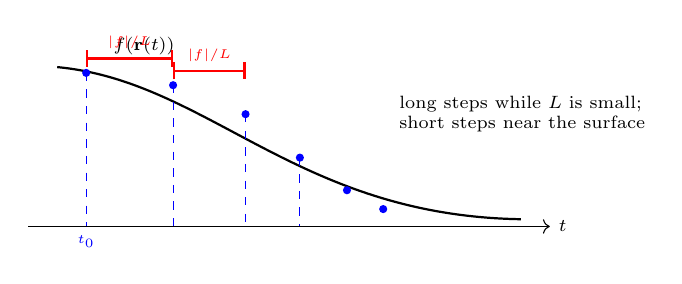
\begin{tikzpicture}[scale=0.92,transform shape]
\draw[->] (0,0) -- (7.2,0) node[right,font=\scriptsize]{$t$};
\draw[thick] (0.4,2.2) .. controls (2.5,2.0) and (3.7,0.15) .. (6.8,0.1);
\node[font=\scriptsize,above] at (1.6,2.25) {$f(\vect{r}(t))$};
\foreach \x/\y in {0.8/2.12, 2.0/1.95, 3.0/1.55, 3.75/0.95, 4.4/0.5, 4.9/0.24}{
  \fill[blue] (\x,\y) circle (1.6pt);
}
\draw[blue,dashed] (0.8,2.12) -- (0.8,0) node[below,font=\tiny]{$t_0$};
\draw[blue,dashed] (2.0,1.95) -- (2.0,0);
\draw[blue,dashed] (3.0,1.55) -- (3.0,0);
\draw[blue,dashed] (3.75,0.95) -- (3.75,0);
\draw[red,thick,|-|] (0.8,2.32) -- node[above,font=\tiny]{$|f|/\Lips$} (2.0,2.32);
\draw[red,thick,|-|] (2.0,2.15) -- node[above,font=\tiny]{$|f|/\Lips$} (3.0,2.15);
\node[font=\scriptsize,align=left,anchor=west] at (5.0,1.55)
  {long steps while $\Lips$ is small;\\ short steps near the surface};
\end{tikzpicture}
\caption{A per-node Lipschitz bound turns the fixed $0.5|f|$ step into
$|f|/\Lips_N$. The step is longer than the old one when the local trilinear
field is smoother than a Lipschitz constant of 2, and shorter (safer) when it is
not. The bound is computed once per revision by the derive pass.}
\label{fig:lipschitz}
\end{figure}

\subsection{Screen-space epsilon is shipped, opt-in}

The world-space epsilon is the main reason grazing rays need hundreds of steps.
At 1\,km and a 60$^\circ$ FOV, one pixel covers about 0.9\,m; the epsilon for a
30-unit leaf is 0.06\,m, fifteen times finer than the screen. The current code
supports a screen-space floor,
\begin{equation}
\epsilon(\vect{p}) = \max\!\left(2\times10^{-3}h,\;\alpha\,t\,\Delta\theta_{\text{px}}\right),
\qquad \alpha\in[0.25,0.5],
\label{eq:eps}
\end{equation}
and refines the accepted hit with a two-step secant clamped to the band
(\fpath{OctreeRaymarch.frag:152--164, 299--323}). The shader already computes
the pixel footprint for the water waves
(\fpath{OctreeRaymarch.frag:1635--1643}), so the quantity is available at no
extra cost. The setting \code{octreeRaymarchScreenEps} defaults to 0
(\fpath{types/Settings.hpp:158--161}); the widget exposes it
(\fpath{widgets/RaymarchWidget.cpp:112--116}). The remaining work is to
validate $\alpha=0.25$ on silhouette and depth-discontinuity scenes and decide
whether to enable it by default. The risk is geometric: a larger epsilon moves
the hit by up to $\alpha$ pixels, which can shift silhouettes and depth. Without
TAA, this can shimmer. \evS\evP

\subsection{Bisection and hit refinement}

The seven-step bisection is exact but expensive, especially with displacement,
where each step evaluates a gradient and up to three texture fetches
(\fpath{OctreeRaymarch.frag:1017--1039}). The field along a short segment inside
one cell is nearly linear, so a false-position (secant) iteration converges in
two or three steps; keeping a bisection safeguard for pathological cells makes
it robust. Step-size relaxation and enhanced sphere tracing pursue the same
goal from the step-law side; B\'an and Valasek review the family and automate
the relaxation parameter \cite{ban2023}. The screen-space path already uses a
secant; extending a safeguarded secant to the ordinary sign-change path is a
small, quality-gated change. \evR\evP

\subsection{Displacement-aware bounds and maxDisp}

With tessellation enabled, the field is $f_{\text{base}}-\text{disp}$ and the
base field's Lipschitz bound no longer applies. The current code handles this
by using the fine tessellation step inside the displacement band
(\fpath{OctreeRaymarch.frag:976--994}). The maximum displacement is derived
from the material at each sample
($\text{maxDisp}=0.5|\code{tessHeightScale}|$); it is not stored per node. If
tessellation becomes a default path, storing \code{maxDisp} in the payload's
reserved \code{normal.w} would replace a per-sample material lookup with a
payload load. That is a small, exact improvement; it does not remove the
texture fetch, which is the real cost. \evP

\subsection{Why an SDF value cache is not viable}

A trilinear sample reads 32\,B of corner data (one 64-byte cache line pair,
usually resident) and performs about 50 floating-point operations. A global
value cache would need a key (three floats plus a node generation), a hash, a
tag comparison, a data load, and a miss path with synchronization. Even in the
best case it is a 300--600 cycle global-memory round trip versus an L1 hit and
50 FLOPs; in the worst case it adds atomics and contention. Its hit rate would
be near zero: different rays sample different positions, and identical
positions are measure-zero; across frames the camera moves and the field
changes. The memory cost (64\,MiB for four million entries) is larger than the
node table it would accelerate. \textbf{Reject.} The corner samples already are
the value cache, and the interpolation is the reuse.

\subsection{Tempting but unsafe: surface-patch bounding boxes}

A per-node bounding box of the zero set, computed from the twelve edge
crossings, would let a ray skip the empty part of a surface cell. For a
trilinear field this is not provably conservative: the zero set can contain a
closed component or a saddle that does not cross a cell edge, so the box of
edge crossings need not contain every surface point. The type-based skip
(Empty/Solid children) and the Lipschitz step are the provably safe
alternatives. Do not ship a surface-patch box without a proof or a conservative
interval-arithmetic bound. \evT

\subsection{Validity after geometry changes}

Every value in the payload is a function of the node's stored corners and cube.
The table builder copies both, and the whole table is rebuilt on any edit, so
the revision invalidates all derived values atomically. There is no need for
per-node versions, and no derived value may outlive its revision. If the
engine later introduces incremental table updates, the payload buffer must be
updated with the same per-node generation; the current design deliberately
does not assume that.

% ============================================================================
\section{Vulkan architecture considerations}
\label{sec:vulkan}
% ============================================================================

\subsection{Fragment versus compute for the primary march}

The primary march must stay in the fragment shader. It writes
\code{gl_FragDepth} and color inside the solid pass, shares the shading body
with the raster path, and (in the RT variant) performs inline ray queries. A
compute wavefront would need a visibility G-buffer, a deferred shading pass, a
depth resolve, and a replacement for the inline ray queries---a new renderer,
not an optimization. The compute budget is therefore reserved for the
once-per-revision payload pass and, if ever built, a tile prepass; the stage
and synchronization rules are those of the Vulkan specification \cite{vkspec}.
\evS

\subsection{Descriptors, bindings and revision visibility}

The raymarch pipeline uses set\,2 bindings 0 (nodes), 1 (roots) and 2 (QEF
payload) (\fpath{RaymarchTable.glsl:37--48}). Bindings 0 and 2 are visible to
the compute and fragment stages because the derive pass reads the nodes and
writes the payload; binding 1 is fragment-only
(\fpath{OctreeRaymarchRenderer.cpp:35--57}). The descriptor layout is already
per-frame; the payload binding follows the same pattern.

The table revision should be pushed in the existing push constant if a
persistent cache is ever added: it has \code{pad0}, \code{pad1}, \code{pad2}
unused (\fpath{OctreeRaymarchRenderer.hpp:56--64}), and the shader's block is
32\,B (\fpath{OctreeRaymarch.frag:94--100}). Adding \code{uint tableVersion}
costs nothing and makes any future cache self-validating. The current QEF
payload does not need it, because the slot's table and payload are produced
together and the flag is set by the same invocation that writes the values.

\subsection{Buffer placement and revision sharing}

The current design allocates one 48\,MiB host-visible node buffer and one
16\,MiB device-local payload buffer per frame slot
(\fpath{OctreeRaymarchRenderer.cpp:250--309}). On an APU this is ordinary DRAM
and the mapped write is cheap. On a discrete GPU the node table is host-memory
read by the fragment shader; without resizable BAR, those reads cross PCIe.
This is the first thing to measure on discrete hardware, and the fix is
independent of any cache:

\begin{enumerate}[leftmargin=1.4em,itemsep=1pt]
\item Allocate the node table in \code{DEVICE_LOCAL} memory and upload it
      through the existing staging ring on a revision change. The table is
      immutable between revisions, so the copy is a one-shot cost.
\item Share one revision buffer across all frames in flight instead of one
      copy per slot. Frames that still reference the previous revision keep it
      alive through the existing deferred-destroy mechanism. This reduces both
      memory (48\,MiB instead of 144\,MiB for the table; 16\,MiB instead of
      48\,MiB for the payload) and upload traffic.
\item If a per-slot descriptor set cannot be repointed safely while in flight,
      keep per-slot descriptor sets but point them all at the same immutable
      buffer; update a slot's set only after its fence.
\end{enumerate}

The same argument applies to the derived payload: one immutable buffer per
revision is enough. The current per-slot payload is simpler and matches the
node-table lifetime; the 32\,MiB saving is an optional follow-up.
\evP

\subsection{Barriers and pass ordering}

The payload pass runs before the march and outside a dynamic-rendering scope.
The shipped sequence is:
\begin{enumerate}[leftmargin=1.4em,itemsep=1pt]
\item \code{HOST_WRITE -> COMPUTE_SHADER_READ} for the node table.
\item \code{HOST_WRITE -> FRAGMENT_SHADER_READ} for the root buffer.
\item Dispatch the payload pass (64 threads per workgroup).
\item \code{COMPUTE_SHADER_WRITE -> FRAGMENT_SHADER_READ} for the payload
      buffer and the record's derived fields.
\item \code{vkCmdBeginRendering} and the fullscreen draw.
\end{enumerate}

The code already records these barriers before \code{vkCmdBeginRendering}
(\fpath{OctreeRaymarchRenderer.cpp:370--436}), and the pass is recorded in the
async solid command buffer, so the compute dispatch fits in the same buffer.
The barrier uses \code{VK_PIPELINE_STAGE_2_COMPUTE_SHADER_BIT},
\code{VK_PIPELINE_STAGE_2_FRAGMENT_SHADER_BIT},
\code{VK_ACCESS_2_SHADER_STORAGE_READ_BIT}/\code{WRITE_BIT}; no
\code{vkDeviceWaitIdle} is needed. \evS

\begin{figure}[t]
\centering
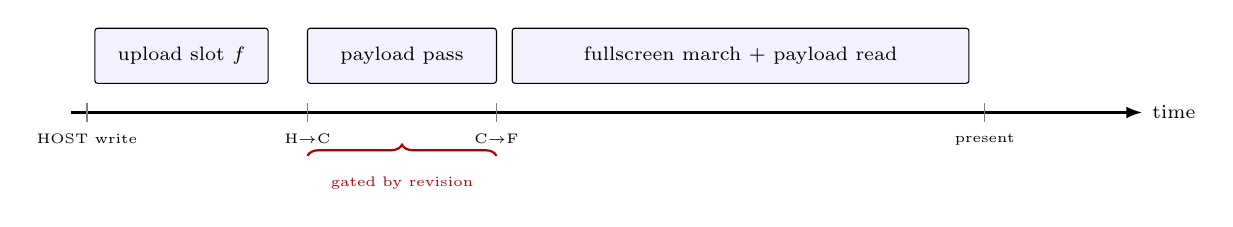
\begin{tikzpicture}[
  x=1cm,y=1cm,
  ev/.style={draw,rounded corners=1pt,align=center,font=\scriptsize,
             minimum height=7mm,fill=blue!5},
  lbl/.style={font=\tiny,anchor=north},
]
\draw[-{Latex[length=2mm]},thick] (0,0) -- (13.6,0)
  node[right,font=\scriptsize]{time};
\foreach \x/\t in {0.2/HOST write, 3.0/H$\to$C, 5.4/C$\to$F, 11.6/present}{
  \draw[gray] (\x,-0.12) -- (\x,0.12);
  \node[lbl] at (\x,-0.15) {\t};
}
\node[ev,minimum width=2.2cm] at (1.4,0.72) {upload slot $f$};
\node[ev,minimum width=2.4cm] at (4.2,0.72) {payload pass};
\node[ev,minimum width=5.8cm] at (8.5,0.72) {fullscreen march + payload read};
\draw[decorate,decoration={brace,amplitude=4pt},thick,red!70!black]
  (3.0,-0.55) -- (5.4,-0.55) node[midway,below=4pt,font=\tiny]{gated by revision};
\end{tikzpicture}
\caption{Per-frame ordering of the payload pass. The pass is skipped when the
slot already holds the current revision; the march itself is unchanged.}
\label{fig:pass}
\end{figure}

\subsection{Subgroups and wave width}

Basic subgroup operations are core in Vulkan 1.1 and GLSL 4.0; the shaders
target Vulkan 1.3 (\fpath{Makefile:298}) and use no subgroup features today.
The reference device is a Radeon 680M (RDNA2), which supports wave32 and
wave64; the implementation selects the wave size, so a design must not assume
one. A 2$\times$2 fragment quad is the only group with a guaranteed spatial
relationship; a subgroup spans an implementation-defined set of lanes and may
migrate between quads. Larger coherent groups are not available in a fragment
shader and would require shared memory, which fragments do not have. Any
subgroup sharing design must therefore be quad-based, and must handle helper
invocations, terminated lanes and quad lanes that leave the primitive. The
expected benefit is small (\cref{sec:B}), so the practical recommendation is to
leave subgroups unused. \evS

\subsection{Register pressure, stack size and occupancy}

\code{RM_MAX_STACK = 16} entries of \code{(uint,float)} are 128\,B per
invocation. The measured table depth is 12, so 16 entries suffice with a small
safety margin; the exact maximum can be computed at build time and pushed.
Dynamic indexing of local arrays in GLSL usually maps to scratch memory, so the
stack is real memory traffic on top of the table reads. Reducing it from the
first edition's 40 entries to 16 is a low-risk change that has already
shipped. \evS

The QEF payload reduces dynamic register pressure indirectly: the ring no
longer runs the solver, so the hit path's live ranges are shorter. The static
fallback still exists in the module, so the compiler must allocate for its
worst-case path unless a no-fallback variant is built. The derive pass is a
separate shader, so its register use does not affect the march.

\subsection{Cache locality and table ordering}

The table is built breadth-first so that the node cap truncates the deepest
level uniformly (\fpath{utils/LocalScene.cpp:595--666}). That is the right
order for construction, but it is not the best order for the march. Siblings
are contiguous, yet consecutive levels are megabytes apart: at the cap, a
depth-11 node and its depth-12 child can be separated by the entire depth-11
level. Adjacent screen pixels at slightly different depths therefore read
widely separated table regions, and the L1/L2 hit rate suffers even though the
rays are coherent.

A spatially coherent permutation (depth-first or Morton order) of the final
node array preserves all semantics: child indices are explicit, and
\code{rmFindNodeAt} only follows them. The builder can keep the BFS cap policy,
then permute the records before upload and rewrite the child indices. The root
record moves to index 0 (or the root entry stores its new index). The cost is
one O($n$) CPU pass and a 4\,B/node remap array; the benefit is that a screen
neighborhood maps to a nearby table region. This is a low-risk, measurable
change and it is independent of any cache. It matters most when the table does
not fit in L2, which is the normal case at 48\,MiB. \evP

The same reasoning applies to access granularity: a 96\,B record spans one
64\,B sector plus a 32\,B sector, while a descent needs only the cube, header
and child information. The compact header already reduced the record from the
old 128\,B; the remaining 96\,B is the sampling record and cannot shrink much
without losing corner data.

\subsection{Workgroup shared memory}

Fragment shaders cannot use workgroup shared memory, so none of the ideas that
depend on cross-pixel shared state (tile cuts, 4$\times$4 or 8$\times$8
traversal, shared candidate lists) can be implemented inside the existing
fragment march. They require a compute prepass. That prepass can use shared
memory freely---a 64-entry cut list is 512\,B, far below the 32--64\,KB
limit---but the prepass is exactly the structure that \cref{sec:C} shows to be
a net loss. The only recommended compute use is the payload pass, which needs
no shared memory because one invocation owns one node; shared memory is used
only for the optional counter aggregation.

\subsection{Divergence and work distribution}

Adjacent pixels have similar step counts in smooth terrain and very different
counts at silhouettes and grazing angles. On a wide wave, the slowest lane in
the wave determines the iteration count; the 1024-step bound exists because
some lanes need about 800. A work queue could compact long rays, but that
requires the wavefront rewrite discussed in F8. The cheaper lever is to reduce
the step count itself (screen-space epsilon, Lipschitz bound, secant
refinement), which helps every lane. \evS\evT

\subsection{Atomics and counters}

Per-ray atomics are too expensive at 921K rays per frame. Aggregate in
workgroup shared memory and issue one atomic per counter per workgroup (64
rays per workgroup gives a 1/64 reduction), then read the buffer after the
slot's fence. The generic SDF renderer's counters use a gate word so the
production path pays only a uniform branch
(\fpath{shaders/renderer/sdf/SdfRenderer.frag:86--96}); the octree variant
should do the same, and the gate should be a compile-time variant or a push
constant, not a per-pixel storage load. \evS\evP

\subsection{Multiple frames in flight and revision hazards}

Three frames are in flight. A revision buffer may be read by frames $N-1$ and
$N-2$ while frame $N$ uses the new one. Two rules keep this safe:
(i) never rewrite a buffer that a pending frame may read---allocate a new
revision and defer-destroy the old one after the last fence; (ii) if a cache
survives across frames, compare its recorded revision with the current one and
reject on mismatch. The current per-slot rewrite is safe because each slot is
fenced before its host write, but it costs three copies. A revision-shared
buffer is the better design if the memory matters. \evS

\subsection{Validation requirements}

The engine's policy is validation-clean execution (\fpath{AGENTS.md}). Any new
buffer, descriptor or pass must be checked with the standard validation layers
and, for the descriptor-indexing-heavy path, GPU-assisted validation. The
payload pass adds a compute write and a fragment read; the barriers above are
the only new synchronization. The counters add a storage buffer with atomics;
the fragment-stage atomics feature is already required by the generic SDF
counters and is checked at init. No new extension is needed: basic subgroups,
storage buffers and compute are core; the inline RT path already uses
\code{VK_KHR_ray_query} \cite{rayquery}. \evS

% ============================================================================
\section{Correctness and invalidation}
\label{sec:correctness}
% ============================================================================

\subsection{What must never happen}

A cache hit must never cause a missed surface, a wrong first hit, a wrong
normal or a material change relative to the uncached march. In this engine
there are four independent ways to violate that:

\begin{enumerate}[leftmargin=1.4em,itemsep=1pt]
\item \textbf{Stale node indices.} The table is rebuilt breadth-first; any edit
      can renumber every node. A cached index from another revision may point
      at a different node with a different cube and corners.
\item \textbf{Unproven prefix.} A cached start node or interval says nothing
      about the space between the origin and the node.
\item \textbf{Stale derived values.} A QEF, normal or material computed from
      old corners can disagree with the current table.
\item \textbf{Floating-point drift.} A cached interval computed with a
      different origin/direction or a different rounding can exclude a
      boundary crossing.
\end{enumerate}

\subsection{Table revision and node index stability}

Node indices are stable within a revision and arbitrary across revisions. The
revision is currently CPU-only; expose it in the push constant before adding
any persistent structure. A cache entry must store the revision it was
produced with and reject on mismatch. Do not use a 16-bit revision: the
current counter is 64-bit and wraps only after $2^{64}$ rebuilds; truncating to
16 bits would create a false-hit window. The QEF payload is exempt because it
is written and consumed within the same slot and revision; its per-node flag
is the validity test. \evS

\subsection{Node lifetime and allocator reuse}

The CPU allocator recycles node memory; the GPU table owns copies, so GPU
lifetime is tied to the buffer, not to the node. This is why the GPU table is
a safe basis for a cache and the CPU node address is not
(\fpath{space/UniqueChangeCollector.hpp:11--30}). Never key a cache by
\code{OctreeNode*} or by \code{node->version}. \evS

\subsection{Floating-point precision}

The march's hit position is a float; the table's cube bounds and corner values
are float copies of the CPU values. Three precautions apply:
\begin{itemize}[leftmargin=1.3em,itemsep=1pt]
\item Expand node boxes by a small epsilon before validating a start point
      ($10^{-6}$ of the node size is enough for float coordinates around
      $10^4$), and clamp $t$ to the interval.
\item Compute the QEF, normal and material in the same GLSL code as the march,
      in a compute pass, not with a separate CPU implementation. The shader's
      \code{precise} qualifiers are part of the result
      (\fpath{SdfCell.glsl:16--22}).
\item Do not quantize the QEF position to half precision. The position feeds
      the hit point, the depth and the material blend; a half-float is not
      bit-exact with the raster path.
\end{itemize}

\subsection{Cache keys and collisions}

The payload cache needs no hash: its key is the node index and its validity is
the per-node flag (and, for a future persistent variant, the table revision).
Any future spatial or temporal cache that uses a hash must store the full
key---node index, revision, and the interval or ray identity it represents---and
treat a tag mismatch as a miss with a root fallback. A collision must never be
accepted as a hit. Do not truncate node indices: the current cap of 524\,288
needs 19 bits and may grow. If a cache uses a smaller tag for bandwidth, the
full key must still be stored alongside it for validation.

\subsection{Safe fallback}

Every cache must have a root-march fallback that is used whenever validation
fails. The fallback should be the current code path, unchanged, so a bug in
the cache degrades performance rather than image correctness. The payload
cache has two fallbacks: the fragment-side QEF solver and the fragment-side
material classifier, both guarded by the payload flags. A start-node or cut
cache would need a root fallback by construction.

\subsection{Image-equality expectations}

\begin{center}
\small
\begin{tabularx}{\linewidth}{@{}lX@{}}
\toprule
Change & Expected image \\
\midrule
F1 carry-forward & Bit-identical: same node, same point, same expression. \\
F2 material/Lipschitz payload & Material expected identical (verify by
  readback; last-bit threshold cases are possible); the Lipschitz step changes
  step positions, so the hit can move by the step-bound difference (still on
  the same surface). Needs an image check, not a hash check. \\
QEF side payload & Position and normal expected identical to the fragment
  solver (verify by readback; cross-module last-bit cases possible). Ring
  barycentrics can shift by the same few ULPs. \\
F3 root order/AABB/clamp & Bit-identical: only skipped intervals that cannot
  contain a hit. \\
F4 compact header & Bit-identical: same child indices, different encoding. \\
F11 screen-space epsilon & Not identical by design: hit moves by up to
  $\alpha$ pixels. Requires a perceptual/image comparison and a quality gate. \\
F13 hit-stack reuse & Bit-identical if the starting ancestor contains the
  query point and the fallback is the root descent. The descent decisions
  depend only on the point. \\
F14 accepted-normal reuse & Bit-identical: same function, same node, same
  point, same module. \\
F15 reciprocal/root hoist & Bit-identical: same arithmetic, computed once. \\
F16 no-fallback variant & Identical only if the derive pass is guaranteed on
  the target; otherwise the fallback must remain. \\
\bottomrule
\end{tabularx}
\end{center}

\subsection{Validation checklist}

Before merging any phase:
\begin{enumerate}[leftmargin=1.4em,itemsep=1pt]
\item No validation errors or warnings in \fpath{logs/run.log}; GPU-assisted
      validation for the descriptor/buffer changes.
\item CPU-side assertion that every child index is in range and that each
      parent's stored children are contiguous (for the compact header).
\item Payload flag present before every payload read; a debug mode that
      forces the flag clear exercises the fallback.
\item Revision check present in every persistent cache.
\item Image comparison against the baseline on the reference scenes.
\item No increase in peak VRAM beyond the budget in \cref{tab:memory}.
\end{enumerate}

% ============================================================================
\section{Performance evaluation plan}
\label{sec:eval}
% ============================================================================

\subsection{Instrument first}

Every quantitative claim in this report is either measured at pass granularity,
derived statically, or inherited from \fpath{qef_gpu.tex}. The engine cannot
presently attribute time inside the march, so the first phase of any remaining
implementation must be instrumentation, not optimization. The generic SDF
renderer already demonstrates the pattern: a per-frame host-visible counter
block, a gate word, and a read after the slot's fence
(\fpath{shaders/renderer/sdf/SdfRenderer.frag:86--96},
\fpath{sdf/types/SdfProfileCounters.hpp}). The octree march should copy it.

\subsection{GPU counters}

A 21-word counter block per frame slot is enough to answer every question in
this report:

\begin{lstlisting}[language=C++,caption={Proposed counter block. 84\,B per slot; aggregate in shared memory, one atomic per workgroup per counter.}]
struct OctreeRaymarchCounters {   // 21 x uint32 = 84 B
    uint32_t rays;              // fragment invocations
    uint32_t rootTests;         // root AABB / interval tests
    uint32_t rootMarches;       // rmMarchRoot calls that entered
    uint32_t nodeVisits;        // distinct node entries (push/pop)
    uint32_t leafIters;         // iterations with leaf == true
    uint32_t nonLeafIters;      // iterations that descend/test a child
    uint32_t fieldEvals;        // march rmTrilinear calls (not bisection)
    uint32_t gradientEvals;     // rmNodeNormal calls
    uint32_t qefSolves;         // sdfCellPosition calls (fallback only)
    uint32_t qefPayloadLoads;   // rmPayload[id].qef reads
    uint32_t ringDescents;      // rmFindNodeAt calls from the hit path
    uint32_t ringCells;         // ring cells considered
    uint32_t ringDuplicates;    // ring cells dropped as duplicates
    uint32_t materialClassifiers; // rmResolveMaterialAt fallback calls
    uint32_t carryHits;         // carry-forward reuses
    uint32_t earlyRoots;        // roots skipped by AABB/order
    uint32_t bisectEvals;       // field evaluations inside bisection
    uint32_t waterSecondary;    // secondary SDF root-list marches
    uint32_t hits;              // accepted primary hits
    uint32_t discardSkips;      // hits rejected by material / back face
    uint32_t enabled;           // CPU-written gate
};
\end{lstlisting}

The gate must be a uniform branch or a specialization constant, not a
per-pixel load of \code{enabled}. Accumulate per workgroup in shared memory and
issue one \code{atomicAdd} per counter per workgroup; at 64 threads per
workgroup this is a 1/64 reduction of atomic traffic. The counters add 252\,B
for three slots and no measurable bandwidth.

\subsection{Timing}

The query pool has 24 slots; slots 0--5 are unused and slots 6--11 are the
existing solid bucket intervals (\fpath{MyApp.cpp:392, 2941--3150}). Use slots
2/3 for a dedicated ``octree march'' interval recorded immediately around
\code{octreeRaymarchRenderer->draw}
(\fpath{MyApp.cpp:3123}). The \code{solid} bucket remains the aggregate. For a
per-section split (march vs hit payload vs shading), use the instrumented
shader-clock variant that the RT profile already uses
(\fpath{shaders/includes/rt/RtProfile.glsl}); the device reports
\code{VK_KHR_shader_clock}. Shader clocks perturb the code; use them only in a
profiling build, never in the acceptance run.

\subsection{Metrics}

\begin{center}
\small
\begin{tabularx}{\linewidth}{@{}lX@{}}
\toprule
Metric & Definition and purpose \\
\midrule
Node visits / ray & \code{nodeVisits / rays}; the traversal workload. \\
Iterations / ray & \code{(leafIters + nonLeafIters) / rays}; the march length. \\
Field evals / iteration & \code{fieldEvals / iterations}; target $\approx 1$ after
  carry-forward. \\
QEF / ray & \code{qefSolves / rays}; target 0 in normal operation. \\
Payload loads / hit & \code{qefPayloadLoads / hits}; target $\le 4$ for a solid
  hit, $\le 12$ for a water pixel. \\
Ring descents / hit & \code{ringDescents / hits}; target $\le 1$ after F13. \\
Bisection / hit & \code{bisectEvals / hits}; target $\le 3$ after secant. \\
Root marches / ray & \code{rootMarches / rays}; target $\le 1$ for primary
  terrain, plus the water lobes. \\
Cache fallback rate & \code{qefSolves / (qefSolves + qefPayloadLoads)}; should be
  zero on supported devices. \\
Bandwidth (estimated) & $\text{visits}\times96$\,B + $\text{ring cells}\times32$\,B. \\
GPU time & \code{solid} p50/p95 plus the dedicated interval; ms. \\
Memory & table + payload + history; MiB; peak VRAM. \\
Image error & max abs diff, SSIM, and a split by material class. \\
\bottomrule
\end{tabularx}
\end{center}

\subsection{Scenes}

The reference scene is the procedural terrain of the first edition: two layers,
524\,288 nodes, 39\% pruned, maximum stored depth 12, a large lake. To avoid
tuning to one scene, add:
\begin{enumerate}[leftmargin=1.4em,itemsep=1pt]
\item \textbf{S0 reference}: the default terrain, static and moving cameras.
\item \textbf{S1 high-frequency}: higher noise amplitude and more surface
      nodes; stresses field sampling and the ring.
\item \textbf{S2 sparse/flat}: few stored nodes; descent-dominated; the best
      case for tile cuts and the worst case for cache overhead.
\item \textbf{S3 water-heavy}: a lake covering more than 30\% of the screen;
      stresses the secondary SDF lobes.
\item \textbf{S4 ground-level grazing}: camera 1--5\,m above the surface; the
      800-step worst case.
\item \textbf{S5 aerial/sky}: mostly sky; stresses root rejection and empty
      space.
\end{enumerate}

\subsection{Comparison matrix}

Build each remaining candidate as a separate toggle or shader variant and
measure it against the same baseline on the same camera path:

\begin{center}
\small
\begin{tabularx}{\linewidth}{@{}llX@{}}
\toprule
Build & Content & Purpose \\
\midrule
B0 & current march & baseline \\
H1 & F13 hit-stack reuse & test the descent saving \\
H2 & F14 accepted-normal reuse & test the duplicate-gradient saving \\
H3 & F15 reciprocal/root hoist & test the per-root overhead \\
H4 & H1+H2+H3 & candidate for shipping \\
H5 & F16 no-fallback variant & test occupancy/instruction footprint \\
H6 & F11 screen epsilon on ($\alpha=0.25$) & quality-gated step saving \\
H7 & F18 revision-shared table/payload & memory and bandwidth \\
A2 & per-pixel previous-node start & test the prefix cost \\
B1 & 2$\times$2 ballot descent & test shared traversal \\
C & per-tile closed-cut prepass & test the tile structure \\
E & previous-frame start for static cameras & test temporal upside \\
\bottomrule
\end{tabularx}
\end{center}

Only H4 is expected to ship. A2, B1, C and E are experiments with the same
acceptance gate; a negative result is a valid outcome and should be documented
so the idea is not retried. The hybrid must be measured with and without each
component (an ablation) so the contribution of F13, F14 and F15 is visible.

\subsection{Configurations and camera paths}

Cross the scenes with: tessellation off/on (the default is off), RT shading
off/on, water on/off, and resolutions 1280$\times$720, 1920$\times$1080 and
2560$\times$1440. Use at least these camera paths:
\begin{itemize}[leftmargin=1.3em,itemsep=1pt]
\item static;
\item slow pan, 5$^\circ$/s;
\item fast pan, 60$^\circ$/s;
\item forward dolly, 1\,m/frame;
\item lateral strafe, 0.5\,m/frame.
\end{itemize}
The engine exposes only a start pose via \code{VULKAN_CAMERA}; there is no
replay recorder. Add a deterministic benchmark path (a test-only hook) so A/B
runs see identical cameras; otherwise the comparison is not repeatable.

\subsection{Procedure and statistics}

For each configuration: 30 warm-up frames, then 300 measured frames, three
runs; report median and p95 GPU time and the counters aggregated over the
measured window. Use the same binary and pipeline cache for A/B; run validation
layers only in the correctness pass (they perturb timing). Compare distributions
with a paired test over frames or simply report the median and p95 with the
run-to-run spread; a 5\% difference is below the noise of an interactive APU
run if the spread is larger, in which case increase the frame count.

\subsection{Acceptance criteria}

A phase is accepted only if all of the following hold:
\begin{enumerate}[leftmargin=1.4em,itemsep=1pt]
\item p95 GPU time for the dedicated octree interval improves by at least 3\%
      on at least two scenes, or the counters show the targeted operation is
      eliminated and the time follows in a second run.
\item The image is bit-identical for F13, F14, F15 and the payload cache; for
      F11 the image difference is within the agreed perceptual budget; for F16
      the fallback is still available on unsupported devices.
\item No validation errors or warnings, including GPU-assisted validation for
      the buffer/descriptor changes.
\item Peak VRAM stays within the budget; the table and payload are not
      duplicated per slot if the revision-sharing change is included.
\item The fallback path is exercised (force the payload flag clear and confirm
      a full QEF solve; force a stack miss and confirm a root descent).
\end{enumerate}

\subsection{Threats to validity}

\begin{itemize}[leftmargin=1.3em,itemsep=1pt]
\item \textbf{Integrated GPU.} The reference machine is an APU with unified
      memory. A host-visible table is cheap here; on a discrete GPU it may
      dominate. Measure the table placement on both.
\item \textbf{Driver and compiler.} AMD's compiler may inline or spill the
      large shader differently after a small change; always compare the same
      driver and check the disassembly/occupancy if a change is unexpectedly
      slow.
\item \textbf{Validation layers.} They can double the frame time; keep them
      out of the timing runs.
\item \textbf{Interactive app.} The application is closed by the user, not by
      the agent (\fpath{AGENTS.md}); the benchmark path must run headless or be
      driven by a deterministic script to be repeatable.
\item \textbf{Scene drift.} The procedural scene is deterministic, but brush
      edits and layer toggles change the table; freeze the scene for the
      measurement and record the table statistics with every run.
\item \textbf{Stale logs.} The first edition's \fpath{logs/run.log} has been
      overwritten. Re-measure the reference scene before comparing with its
      numbers; do not treat the historical solid-bucket times as current.
\end{itemize}

% ============================================================================
\section{Comparison and ranking}
\label{sec:ranking}
% ============================================================================

\subsection{Scored comparison}

Table~\ref{tab:scores} assigns scores from 1 (low) to 5 (high) for expected
benefit, implementation complexity and risk. Benefit is relative to the
raymarch time; complexity includes shader, CPU and synchronization work; risk
includes image correctness, validation and maintenance. The scatter plot in
Figure~\ref{fig:scatter} places the remaining candidates; the shaded region is
the ``do first'' quadrant.

\begin{table}[t]
\centering
\small
\caption{Scored ranking of the remaining candidates. Scores are judgements
from the analysis, not measurements. Shipped items are listed in
\cref{tab:approaches} and are not ranked.}
\label{tab:scores}
\begin{tabular}{@{}lcccl@{}}
\toprule
Candidate & Benefit & Complexity & Risk & Rank / note \\
\midrule
F13 hit-stack reuse & 4 & 2 & 1 & 1: exact, zero memory \\
F14 accepted-normal reuse & 3 & 1 & 1 & 2: exact, tiny \\
F15 reciprocal/root hoist & 2 & 1 & 1 & 3: exact, tiny \\
F16 no-fallback variant & 3 & 3 & 2 & 4: occupancy experiment \\
F11 screen epsilon on & 4 & 2 & 3 & 5: quality-gated \\
F18 revision sharing & 2 & 3 & 2 & 6: memory only \\
F5 parametric child & 2 & 3 & 2 & 7: small, optional \\
F17 maxDisp payload & 1 & 2 & 1 & 8: tessellation only \\
D water secondary & 2 & 4 & 3 & 9: rendering architecture, not cache \\
B1 2$\times$2 quad sharing & 2 & 4 & 3 & 10: low ceiling \\
C tile closed cut & 1 & 5 & 4 & 11: net loss likely \\
A2/A3 per-ray history & 1 & 4 & 5 & 12: prefix unsound \\
E temporal & 1 & 5 & 5 & 13: motion invalidates \\
\bottomrule
\end{tabular}
\end{table}

\begin{figure}[t]
\centering
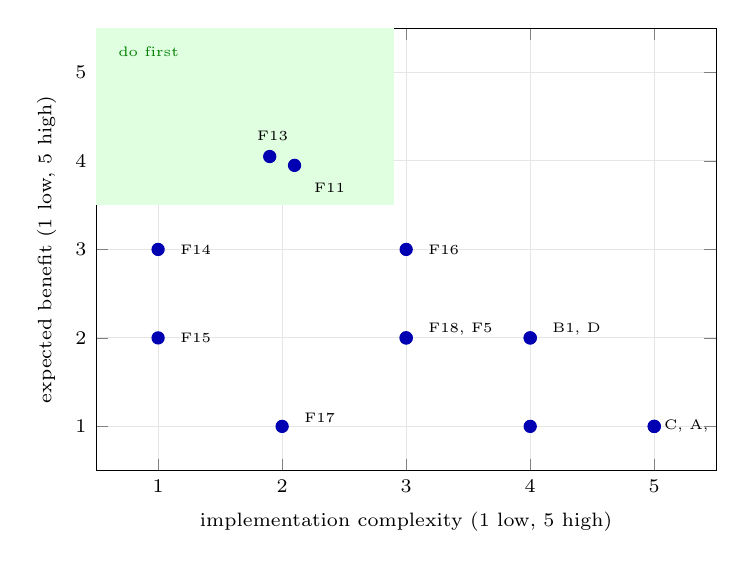
\begin{tikzpicture}[
  pt/.style={circle,inner sep=1.6pt,fill=blue!70!black},
  lbl/.style={font=\tiny,anchor=west},
]
\begin{axis}[
  width=0.78\linewidth,height=7.2cm,
  xlabel={implementation complexity (1 low, 5 high)},
  ylabel={expected benefit (1 low, 5 high)},
  xmin=0.5,xmax=5.5,ymin=0.5,ymax=5.5,
  xtick={1,2,3,4,5},ytick={1,2,3,4,5},
  grid=major,grid style={gray!20},
  tick label style={font=\scriptsize},label style={font=\scriptsize},
]
\fill[green!12] (axis cs:0.5,3.5) rectangle (axis cs:2.9,5.5);
\node[font=\tiny,green!50!black,anchor=north west] at (axis cs:0.6,5.4) {do first};
\addplot[only marks,mark=*,mark size=2.2pt,blue!70!black] coordinates {
 (1.9,4.05) (1,3) (1,2) (3,3) (2.1,3.95) (3,2) (3,2) (2,1) (4,2) (4,2) (5,1) (4,1) (5,1)
};
\node[lbl,anchor=south west] at (axis cs:1.72,4.12) {F13};
\node[lbl] at (axis cs:1.1,3.0) {F14};
\node[lbl] at (axis cs:1.1,2.0) {F15};
\node[lbl] at (axis cs:3.1,3.0) {F16};
\node[lbl,anchor=north west] at (axis cs:2.18,3.86) {F11};
\node[lbl] at (axis cs:3.1,2.1) {F18, F5};
\node[lbl] at (axis cs:2.1,1.1) {F17};
\node[lbl] at (axis cs:4.1,2.1) {B1, D};
\node[lbl] at (axis cs:5.0,1.0) {C, A, E};
\end{axis}
\end{tikzpicture}
\caption{Benefit versus complexity for the remaining candidates. The shaded
quadrant is the recommended first wave: F13, F14 and F15, with F11 as the
quality-gated follow-up. The low-benefit/high-complexity corner is the ``do not
build'' region.}
\label{fig:scatter}
\end{figure}

\subsection{Why the ranking is not the conventional one}

A conventional ray-tracing optimization would start with the acceleration
structure: caches, packets, tiles, temporal reprojection. That ordering assumes
traversal is the bottleneck. In this engine it is not. Three facts invert it:

\begin{enumerate}[leftmargin=1.4em,itemsep=1pt]
\item The traversal is a single-child descent with an ancestor stack; it does
      not test eight children per node and does not restart from the root on a
      pop. The per-ray descent is a few hundred operations.
\item The per-node QEF/material solve, which the first edition identified as
      the largest repeated cost, is now cached. The remaining repeated
      traversal is the hit path's five-to-fifteen root descents, and it is
      intra-ray, not inter-ray.
\item Shading dominates the solid pass. No traversal cache can remove the
      texture fetches, shadow lookups or RT rays.
\end{enumerate}

The external literature still supports the scepticism about packet-style
sharing on GPUs: per-ray traversal outperformed packet traversal even for
primary rays, and packet traversal was a factor 1.7--2.4 below the simulated
optimum \cite{aila2009}; stackless traversal was 20--31\% slower on a GPU
\cite{afra2014}. Those results are for BVHs, not SDF octrees, but the mechanism
(SIMT divergence and work distribution) applies.

\subsection{Expected combined effect}

The remaining changes overlap. F13 removes root descents, which makes the
remaining field samples and shading relatively more important; F14 removes a
gradient per water or displaced hit; F15 removes a few divisions per root
march. A rough composition (not a measurement) is:
\begin{itemize}[leftmargin=1.3em,itemsep=1pt]
\item F13: removes up to five root descents per solid hit and up to fifteen per
      water pixel; perhaps 3--10\% of march traversal arithmetic.
\item F14: removes one gradient per water hit, one per displaced hit, and one
      on the ring fallback; perhaps 1--4\% of the hit path.
\item F15: removes three divisions and one box test per root march; below 1\%.
\end{itemize}
Multiplying these as independent fractions is wrong; the counters in
\cref{sec:eval} must measure the combination. A plausible range is a 3--12\%
faster march; through Amdahl (\cref{tab:amdahl}) that is a 1--4\% solid-pass
improvement if the march is 30--40\% of the pass. These are targets to test,
not promises. \evT

The first edition's larger estimate (1.5--2.2$\times$ for the march) belonged
to the payload cache, which has already shipped. The remaining opportunities
are smaller because the big repeated cost is gone.

% ============================================================================
\section{Recommended architecture}
\label{sec:rec}
% ============================================================================

\subsection{Overview: three layers, only one of which is a cache}

The recommendation is a layered design in which only the payload layer stores
data across invocations. The other two are state that the march already has or
can derive for free. The payload layer is already shipped; the remaining work
is in layers 1 and 2.

\begin{description}[leftmargin=1.2em,itemsep=3pt]
\item[Layer 0 --- node payload cache (shipped).] A once-per-revision compute
  pass derives, for every stored node, the QEF position/normal, the resolved
  material and the Lipschitz bound. The march and the hit path read them. This
  is the only persistent cache. It has a 100\% hit rate, no collisions, a
  per-node validity flag, and no image change (the values are computed by the
  same GLSL code).
\item[Layer 1 --- intra-ray state reuse.] Carry the last field sample forward
  (shipped), hoist the ray reciprocal (shipped), keep the ancestor stack
  (shipped, 16 entries), and reuse the march stack for the hit-time node
  queries (remaining). Also return the accepted hit normal from the march so
  the water/displacement paths do not solve it again (remaining). No memory,
  no invalidation, bit-exact.
\item[Layer 2 --- per-root reuse.] Compute a tight surface AABB per layer,
  test it before the root cube, order roots by interval entry, and clamp each
  subsequent march to the nearest hit so far (shipped). The water lobes reuse
  the same root entries and AABBs; they cannot reuse the primary intervals
  because their directions differ.
\end{description}

Figure~\ref{fig:arch} shows the current data flow and the remaining intra-ray
path. The optional record compaction (already shipped) and the optional
screen-space epsilon (shipped, opt-in) are marked for context.

\begin{figure}[t]
\centering
\resizebox{\linewidth}{!}{%
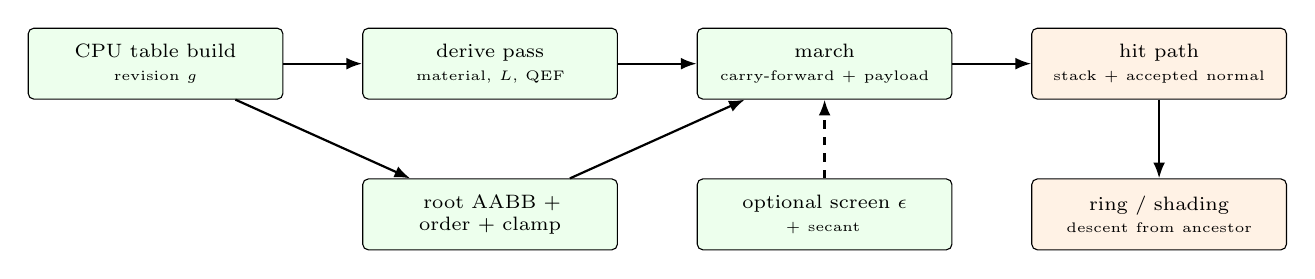
\begin{tikzpicture}[
  box/.style={draw,rounded corners=2pt,align=center,font=\scriptsize,
              minimum height=9mm,text width=30mm,fill=blue!5},
  ship/.style={box,fill=green!7},
  rem/.style={box,fill=orange!10},
  arr/.style={-{Latex[length=2mm]},thick},
  lbl/.style={font=\tiny,fill=white,inner sep=1pt}
]
\node[ship] (table) {CPU table build\\\tiny revision $g$};
\node[ship,right=10mm of table] (payload) {derive pass\\\tiny material, $\Lips$, QEF};
\node[ship,right=10mm of payload] (march) {march\\\tiny carry-forward + payload};
\node[rem,right=10mm of march] (hit) {hit path\\\tiny stack + accepted normal};
\node[rem,below=10mm of hit] (ring) {ring / shading\\\tiny descent from ancestor};
\node[ship,below=10mm of payload] (root) {root AABB + order + clamp};
\node[ship,below=10mm of march] (eps) {optional screen $\epsilon$\\\tiny + secant};

\draw[arr] (table) -- (payload);
\draw[arr] (payload) -- (march);
\draw[arr] (march) -- (hit);
\draw[arr] (hit) -- (ring);
\draw[arr] (root) -- (march);
\draw[arr] (table) -- (root);
\draw[arr,dashed] (eps) -- (march);
\end{tikzpicture}}
\caption{Current data flow (green) and the remaining intra-ray reuse (orange).
The payload pass is rebuilt once per revision and read by the march through
set\,2 binding 2; the hit path receives the march stack and the accepted normal
instead of restarting from the root.}
\label{fig:arch}
\end{figure}

\subsection{Return the accepted hit normal}

\code{rmMarchRoot} already computes the analytic normal in \code{rmHitAllowed}
for every candidate hit. Add an output parameter (or a small hit struct) that
carries the accepted normal and material out of the march. Then:
\begin{itemize}[leftmargin=1.3em,itemsep=1pt]
\item the water branch in \code{main} uses the returned normal as the SDF
      interface normal instead of calling \code{rmNodeNormal} again;
\item \code{rmResolveHitShading} uses it as the initial \code{sdfNormal} for
      the displacement fixed point and as the ring-fallback normal;
\item the solid path keeps using the ring's barycentric normal when available;
      the returned normal is only the fallback.
\end{itemize}
The call arguments are identical (same node, same point, same module), so the
result is bit-identical. The change removes one gradient per water hit, one per
displaced hit, and one when the ring could not reconstruct a normal. It is the
smallest exact change in the report. \evP

\subsection{Return the ancestor stack and reuse it}

Move the march stack from a local array in \code{rmMarchRoot} to a
file-scope invocation-local array (\code{rmStackNode}, \code{rmStackExit},
\code{rmStackDepth}) and return the hit depth. Add a helper:

\begin{lstlisting}[language=C++,caption={Ancestor-start descent. The deepest containing ancestor is a safe starting point; the root is the fallback.}]
uint rmFindNodeFromStack(uint root, vec3 pos) {
    // Start at the deepest stacked ancestor whose cube contains pos.
    for (int d = rmStackDepth - 1; d >= 0; --d) {
        uint n = rmStackNode[d];
        vec3 mn = rmNodeMin(n);
        if (all(lessThanEqual(mn, pos)) &&
            all(lessThanEqual(pos, mn + vec3(rmNodeSize(n)))))
            return rmDescendFrom(n, pos);   // same loop as rmFindNodeAt
    }
    return rmFindNodeAt(root, pos);         // fallback
}
\end{lstlisting}

\code{rmResolveHitShading} and \code{rmBlendAtHit} call this helper instead of
\code{rmFindNodeAt}. The hit node itself contains the hit point; it can be
tested first, before the stack, to cover the base point. The result is exact
because the descent from a containing ancestor makes the same child choices as
the descent from the root; only the prefix is skipped, and the prefix is
exactly the ancestors' path. If the point is outside every stacked ancestor
(the ring can extend into a neighboring subtree), the root fallback runs.
The helper removes up to five descents per solid hit and up to fifteen per
water pixel. \evP

\paragraph{Stack size and aliasing.} The stack is 16 entries (128\,B). Making
it file-scope does not increase its size; it only extends its lifetime to the
hit path. The march must reset \code{rmStackDepth} on entry and on every discard
path, exactly as the local stack is reset by scoping. The material cache
\code{rmBrushNode}/\code{rmBrushValue} is already file-scope and invocation-local,
so the pattern exists.

\subsection{Root, reciprocal and interval reuse}

The caller already computes \code{invRd} for the root AABB tests
(\fpath{OctreeRaymarch.frag:1468}) and \code{rmMarchRoot} recomputes it
(\fpath{OctreeRaymarch.frag:812}). Pass \code{invRd} into \code{rmMarchRoot}
(and into the solid-root helper) and, when the caller already tested the root
cube rather than the surface AABB, pass the root entry $t_0$ so the march can
skip the duplicate slab test. The surface AABB and the root cube are different
boxes; keep both tests when the rejection box is tighter, but reuse the
reciprocals. The change removes three divisions and one box test per root
march. \evP

\subsection{Payload lifecycle and memory}

The shipped payload is per slot. Two optional changes reduce memory and upload
traffic without touching the march:
\begin{enumerate}[leftmargin=1.4em,itemsep=1pt]
\item Make the node table device-local and upload it once per revision through
      the staging ring. The table is immutable between revisions.
\item Share one revision's table and payload across the three slots, with
      deferred destroy for the previous revision and a descriptor update after
      the slot fence.
\end{enumerate}
The combined saving is 96\,MiB (table) plus 32\,MiB (payload). The risk is a
lifetime bug, not an image bug; a debug mode that forces a revision change
while two frames are in flight exercises it. On the APU the bandwidth benefit
is modest; on a discrete GPU it is the first thing to do. \evP

\subsection{Optional no-fallback variant}

The QEF solver and classifier remain in the fragment module for robustness.
For devices where the derive pass is guaranteed, a separate fragment variant
(or a specialization constant that selects a module without the fallback) can
remove the solver's register pressure and instruction-cache footprint. This is
a measured experiment: build the variant, compare the disassembly/occupancy
and the p95 time, and keep the fallback variant as the default. Do not make the
payload a correctness dependency. \evP

\subsection{What not to build}

For clarity, the recommendation excludes:
\begin{itemize}[leftmargin=1.3em,itemsep=1pt]
\item persistent per-pixel temporal start nodes or stacks (prefix unsound;
      motion invalidates);
\item per-tile cut lists or per-tile ancestor chains (net loss; see
      \cref{sec:C});
\item 4$\times$4/8$\times$8 shared traversal or packet traversal (low ceiling,
      high complexity, contrary GPU evidence);
\item stackless traversal (slower on GPUs for this use);
\item ray sorting, wavefront or work queues for primary visibility (new
      renderer; contradicts the architecture constraint);
\item a global SDF value cache (no reuse; larger than the table);
\item a surface-patch bounding box without a conservative proof;
\item a separate secondary-ray octree cache (the TLAS is the right structure,
      and the SDF lobes are shading-bound).
\end{itemize}

\subsection{Risks and mitigations}

\begin{center}
\small
\begin{tabularx}{\linewidth}{@{}lXl@{}}
\toprule
Risk & Mitigation & Owner phase \\
\midrule
Stack lifetime leak into the hit path & Reset depth on entry and every discard;
  debug assertion that the hit node is in the stack & 1 \\
Stale ancestor cube & Validate containment per level; root fallback & 1 \\
Accepted normal mismatch & Same function, same arguments; image hash check & 1 \\
Payload flag/format drift & Shared headers and static asserts; readback test & 2 \\
Revision-shared lifetime & Deferred destroy + fence-gated descriptor update & 2 \\
Occupancy regression from no-fallback variant & A/B p95 and disassembly;
  keep the fallback default & 2 \\
Image shift from screen-space $\epsilon$ & Setting, image comparison, start at
  $\alpha=0.25$ & 3 \\
Counters perturbing the result & Gate off in acceptance runs; shared-memory
  aggregation & 0 \\
\bottomrule
\end{tabularx}
\end{center}

% ============================================================================
\section{Phased implementation and benchmarking plan}
\label{sec:plan}
% ============================================================================

The plan is ordered by benefit per unit of risk. Each phase has a gate; a phase
that does not pass its gate is reverted rather than carried forward. No phase
changes the octree representation or the Vulkan pipeline structure.

\begin{table}[t]
\centering
\scriptsize
\caption{Phased plan for the remaining work. ``Image'' states the expected
image relation to the baseline. Gates are measured on the counters of
\cref{sec:eval}.}
\label{tab:plan}
\begin{tabularx}{\linewidth}{@{}p{0.8cm}p{4.2cm}p{2.3cm}p{1.9cm}X@{}}
\toprule
Phase & Work & Image & Gate & Rollback / notes \\
\midrule
0 & Counters, revision in push constant, dedicated timer slot, deterministic
  camera path & identical & baseline counters + p95 established &
  instrumentation only; no visual change \\
1 & F13 hit-stack reuse; F14 accepted-normal reuse; F15 reciprocal/root hoist &
  identical & $\ge3\%$ p95 on S0/S3 or ring descents/hit $\le1$ &
  each item separable; revert the one that regresses \\
2 & F16 no-fallback variant; F18 revision-shared table/payload; F17 maxDisp &
  identical & $\ge2\%$ p95 for F16 or $\ge64$\,MiB saved for F18 &
  keep the fallback variant; lifetime test \\
3 & F11 screen epsilon default validation ($\alpha=0.25$) & within budget &
  $\ge10\%$ p95 on S1/S4; image approved & feature flag; default off until
  approved \\
4 & Optional research: F5 parametric child; water half-res/RT; B1/C only if
  counters show descent $>15\%$ & exact for F5 & only if counters justify;
  otherwise stop & stop after two negative experiments \\
\bottomrule
\end{tabularx}
\end{table}

\subsection{Phase 0: instrumentation (1--2 days)}

Add the counter block and the revision push constant, bracket the draw with a
new timestamp interval, and add a deterministic camera path for A/B. Produce a
baseline report with the metrics of \cref{sec:eval} for S0--S5. Do not optimize
yet. The expected outcome is that \code{qefSolves/ray} is zero (or the fallback
rate is explained), \code{qefPayloadLoads/hit} is near four, and
\code{ringDescents/hit} is near five for solids and near fifteen for water. If
they do not, re-derive the cost model before phase 1.

\subsection{Phase 1: intra-ray hit reuse (2--4 days)}

Implement the stack reuse, the accepted-normal return and the reciprocal/root
hoist. All are bit-exact. The stack reuse depends on moving the local stack to
file scope and resetting it on every exit path; add a debug assertion that the
hit node's ancestors are present. Run the counters: \code{ringDescents/hit}
should fall toward one, and the dedicated interval should improve. If the
counters show no change, the hit path is already dominated by shading and the
phase should be reverted rather than carried.

\subsection{Phase 2: payload lifecycle (3--5 days)}

Add the no-fallback variant and the revision-sharing option. The no-fallback
variant must keep the fallback pipeline available for devices where the derive
pass fails; the revision-sharing option must defer-destroy the previous
revision and update descriptors only after the slot fence. Measure memory and
bandwidth; on the APU the bandwidth benefit may be neutral, which is acceptable
as long as memory falls.

\subsection{Phase 3: screen-space epsilon validation (2--4 days)}

The implementation is already shipped behind \code{octreeRaymarchScreenEps};
the work is validation, not implementation. Compare images on S1 and S4 at
$\alpha=0.25$ and, if acceptable, $\alpha=0.5$. Measure the step-count
reduction. If the difference is not visually acceptable, reduce $\alpha$ or
leave the default at zero; the rest of the architecture does not depend on it.

\subsection{Phase 4: research (time-boxed)}

Run F5 (parametric child selection) on S0, the water half-resolution/RT
experiments on S3, and B1/C only if the counters show the descent is more than
15\% of the march. If the experiments do not clear a 3--5\% gate, stop; the
analysis says they will not.

\subsection{Expected cumulative outcome}

The remaining phases are designed so that each can ship independently. The
expected range is a 3--12\% faster march and a 1--4\% faster solid pass, with
the largest contributions from F13 and F14. These are targets derived from the
static model, not measured results; the gates exist precisely because the model
may be wrong. \evT

% ============================================================================
\section{Conclusion}
% ============================================================================

The investigation set out to find the most effective way to avoid repeatedly
traversing the same octree hierarchy for coherent primary and secondary rays.
The first edition's answer was to cache the per-node SDF-derived payload, and
that answer was right: the current engine stores the resolved material, the
inverse Lipschitz bound and the QEF position/normal once per revision, and the
march and hit ring read them. The QEF analysis in \fpath{qef_gpu.tex} isolated
the remaining per-frame solves and led to the 32\,B/node side buffer; the
subsequent changes made the ring a payload-read path. In normal operation the
march performs no QEF solve at all.

The second iteration's answer to the same question is narrower. What remains
is not a persistent cache but intra-ray state reuse. The march holds the
ancestor chain of the hit node, yet the hit path restarts from the root five
times for a solid hit and up to fifteen times for a water pixel. The march also
computes the accepted hit's analytic normal, which the water and displacement
paths solve again. Both are exact, zero-memory fixes: return the stack and the
normal from the march and reuse them. Hoisting the ray reciprocals and the root
interval removes a smaller duplicate. A no-fallback variant and revision-shared
buffers are optional follow-ups, not requirements.

The requested spatial and temporal caches remain below these changes.
Per-pixel temporal starts are unsound without a closed cover and are
invalidated by ordinary camera rotation; tile cut lists cost more to build and
walk than the descent they replace; neighboring-ray sharing has a low ceiling
because the expensive per-sample work and shading cannot be shared; and a
separate secondary-ray cache duplicates the triangle TLAS. The external
literature is consistent with this: per-ray traversal has been measured faster
than packet traversal on GPUs, and stackless traversal slower, for the ray
classes that resemble this march.

The report does not claim a measured speed-up. It provides the updated cost
model, the counter design, the benchmark matrix and the phased gates needed to
turn the remaining model into measurements. The first action is phase~0:
instrument the march, confirm the hit-path descents and the payload fallback
rate, and then implement the intra-ray reuse in that order.

% ============================================================================
\appendix
\section{Evidence map}
\label{app:evidence}
% ============================================================================

\begin{footnotesize}
\begin{longtable}{@{}p{5.9cm}p{9.4cm}@{}}
\caption{Every architectural fact used in this report, with its source. Line
numbers refer to the current tree. The first edition's \fpath{logs/run.log}
statistics are historical and are marked as such.}\\
\toprule
Fact & Source \\
\midrule
\endfirsthead
\toprule
Fact & Source \\
\midrule
\endhead
\bottomrule
\endfoot
Node record is 96\,B, six \code{vec4}s; child base + mask &
  \fpath{utils/OctreeRaymarchTable.hpp:26--39},
  \fpath{shaders/includes/octree/RaymarchNodeRecord.glsl:20--40} \\
QEF payload is 32\,B, two \code{vec4}s &
  \fpath{utils/OctreeRaymarchTable.hpp:66--73},
  \fpath{shaders/includes/octree/RaymarchPayload.glsl:11--15} \\
Root entry is 48\,B; node, layer id, kind, surface AABB &
  \fpath{utils/OctreeRaymarchTable.hpp:49--60},
  \fpath{RaymarchTable.glsl:28--35} \\
Flags: leaf bit0, payload bit1, QEF bit2, pruned 8--15, child type 16--31 &
  \fpath{RaymarchNodeRecord.glsl:30--40},
  \fpath{OctreeRaymarchTable.hpp:80--96} \\
Child resolution is base + bitCount(mask below slot) &
  \fpath{RaymarchTable.glsl:58--67} \\
Only surface nodes stored; non-surface children typed in the parent &
  \fpath{utils/LocalScene.cpp:498--718} \\
Breadth-first build; child cap prunes deepest surface children &
  \fpath{utils/LocalScene.cpp:595--666} \\
Surface AABB is the union of stored cells plus pruned child cubes &
  \fpath{utils/LocalScene.cpp:596--700} \\
Node cap 524\,288; root cap 256; 3 slots &
  \fpath{vulkan/renderer/octree/OctreeRaymarchRenderer.hpp:42--54} \\
Per-slot node/root buffers are host-visible, coherent, mapped &
  \fpath{OctreeRaymarchRenderer.cpp:258--309} \\
QEF payload is device-local, 32\,B/node, dummy when derive unavailable &
  \fpath{OctreeRaymarchRenderer.cpp:272--281} \\
Upload is a full \code{memcpy} per revision; derive marked per slot &
  \fpath{OctreeRaymarchRenderer.cpp:311--339} \\
Derive pass writes material, $1/\Lips$, QEF position/normal &
  \fpath{OctreeDerive.comp:52--78} \\
Set-2 bindings 0/1/2; 0 and 2 are compute+fragment &
  \fpath{OctreeRaymarchRenderer.cpp:35--57},
  \fpath{RaymarchTable.glsl:37--48} \\
Host and compute barriers before the march &
  \fpath{OctreeRaymarchRenderer.cpp:370--436} \\
Revision is CPU-only; debounce 0.4\,s; immediate after a brush &
  \fpath{MyApp.cpp:5184--5225, 5709--5712} \\
Node fields: \code{sdf[8]}, type, brush, lod, \code{uint version} &
  \fpath{space/OctreeNode.hpp:11--33} \\
\code{version} incremented only for chunk nodes; never read &
  \fpath{space/Octree.cpp:913--915} \\
Allocator recycles addresses; version-keyed dedup is unsound &
  \fpath{space/UniqueChangeCollector.hpp:11--30} \\
\code{RM_MAX_STEPS}=1024, \code{RM_MAX_STACK}=16, \code{RM_MAX_ROOTS}=16,
  \code{RM_BISECT_STEPS}=7 &
  \fpath{OctreeRaymarch.frag:135--150} \\
Grazing rays can need about 800 steps &
  \fpath{OctreeRaymarch.frag:136--139} \\
Hit epsilon world-space floor and optional screen-space widening &
  \fpath{OctreeRaymarch.frag:152--164} \\
Material payload read; QEF fallback &
  \fpath{OctreeRaymarch.frag:203--221} \\
QEF position/normal payload reads; fallback &
  \fpath{OctreeRaymarch.frag:183--235} \\
Lipschitz step and inverse bound &
  \fpath{OctreeRaymarch.frag:996--1004},
  \fpath{RaymarchMaterial.glsl:39--53} \\
Carry-forward sample &
  \fpath{OctreeRaymarch.frag:826--835, 943--950, 1041--1050} \\
Child descent, skip, pruned fallback, stack, displacement suspension &
  \fpath{OctreeRaymarch.frag:844--937} \\
Hit acceptance and analytic normal &
  \fpath{OctreeRaymarch.frag:801--805} \\
Hit ring: four cells, payload loads, barycentric blend &
  \fpath{OctreeRaymarch.frag:482--729} \\
Hit shading: base point, root descent, ring, normal fallback &
  \fpath{OctreeRaymarch.frag:1066--1117} \\
Root AABB/order/clamp in \code{main} &
  \fpath{OctreeRaymarch.frag:1166--1179, 1470--1515} \\
Water lobes: two solid-root list marches &
  \fpath{OctreeRaymarch.frag:1184--1245, 1343--1445} \\
Water normal smoothing uses the ring when curved &
  \fpath{OctreeRaymarch.frag:1531--1557} \\
RT water resolve and TLAS path &
  \fpath{RtReflection.glsl:179--300} \\
RT shading selector &
  \fpath{vulkan/renderer/SceneRenderer.cpp:3132--3153} \\
Defaults: tessellation off, raymarch off, screen eps 0, RT off &
  \fpath{types/Settings.hpp:147, 157, 161, 187, 197} \\
Solid shading cost (three materials, maps, CSM, RT) &
  \fpath{shaders/includes/solid/SolidSurface.glsl:86--260} \\
Generic SDF counter precedent &
  \fpath{shaders/renderer/sdf/SdfRenderer.frag:86--96},
  \fpath{sdf/types/SdfProfileCounters.hpp} \\
Query pool has 24 slots; 0--5 unused; solid uses 6--11 &
  \fpath{MyApp.cpp:392, 2941--3150} \\
Push constant has three unused words &
  \fpath{OctreeRaymarchRenderer.hpp:56--64} \\
Shaders target Vulkan 1.3 &
  \fpath{Makefile:294--302} \\
QEF SPIR-V counts and per-frame solve estimates &
  \fpath{docs/qef_gpu.tex}, tables 2--4 \\
Reference table: 524\,288 nodes, 2 layers, 39.0\% pruned, depth 12,
  0 infinite corners & first-edition recorded run (historical) \\
Reference roots: 15\,360 and 30\,720 units & first-edition recorded run \\
Reference pass times: solid 141.65--505.67\,ms; others $\le1.7$\,ms &
  first-edition recorded run (historical) \\
Device and enabled features & first-edition \fpath{logs/run.log:1--9};
  current device reports the same extensions \\
\end{longtable}
\end{footnotesize}

% ============================================================================
\section{Instrumentation and push-constant sketch}
\label{app:counters}
% ============================================================================

\begin{lstlisting}[language=C++,caption={Push constant update. The three pad words already exist; no ABI change.}]
struct PushConstants {
    glm::vec4 viewport;
    uint32_t  rootCount;
    uint32_t  tableVersion;   // was pad0
    uint32_t  nodeCount;      // was pad1
    uint32_t  flags;          // was pad2: bit0 counters, bit1 payload valid
};
\end{lstlisting}

\begin{lstlisting}[language=C++,caption={GLSL side. Binding numbers are placeholders; binding 2 is the QEF payload.}]
layout(std430, set = 2, binding = 2) readonly buffer RaymarchPayload {
    RaymarchPayload rmPayload[];
};
layout(std430, set = 2, binding = 3) buffer RaymarchCounters {
    uint rmCounters[21];
};

shared uint shCounters[21];

void rmCount(uint idx) {
    if ((pc.flags & 1u) != 0u) atomicAdd(shCounters[idx], 1u);
}
// At the end of main(), if the invocation is lane 0 of the workgroup,
// flush the 21 shared counters with one atomicAdd each.
\end{lstlisting}

The acceptance run uses the gate off; the profiling build uses it on. The
counter buffer is host-visible and read after the slot's fence, exactly like
\fpath{SdfRenderer::readProfile}.

% ============================================================================
\section{Derivations}
\label{app:derivations}
% ============================================================================

\subsection{Trilinear gradient bound}

With the notation of \cref{sec:sdfcache}, the trilinear interpolant is
\begin{equation}
f(\vect{l})=\sum_{i,j,k\in\{0,1\}} d_{ijk}\,B_i(l_x)B_j(l_y)B_k(l_z),
\end{equation}
where $B_0(t)=1-t$, $B_1(t)=t$. Differentiating in $l_x$,
\begin{equation}
\partial_{l_x} f=\sum_{j,k}(d_{1jk}-d_{0jk})B_j(l_y)B_k(l_z),
\end{equation}
and because $B_jB_k\ge0$ and $\sum_{j,k}B_jB_k=1$,
$|\partial_{l_x}f|\le\max_{j,k}|d_{1jk}-d_{0jk}|=\Delta_x$.
The chain rule gives $\partial_x f=\partial_{l_x}f/h$, and the Euclidean norm
of the gradient is bounded by \eqref{eq:lipschitz}.

\subsection{Safe step and the 0.5 factor}

For a field with Lipschitz bound $\Lips$, the distance from a point with value
$f>0$ to the zero set is at least $f/\Lips$ (Hart's signed-distance bound
\cite{hart1996}). Advancing by that amount cannot cross the surface, so
\eqref{eq:step} is safe. The current code uses $f/2$ when no payload is
available, i.e.\ it assumes $\Lips\le2$. For a trilinear interpolation of a
1-Lipschitz field, $\Lips\le\sqrt3$, so the fixed step is conservative by up to
15.5\%; for fields with corner differences larger than the cell size it is not
conservative. The per-node bound is both faster and safer, and it is now
shipped.

\subsection{Closed-cut exactness}

\begin{theorem}[Restated]
If $\mathcal{S}$ is a closed cut of the tile cone and every ray's interval is
covered by the node intervals, marching the nodes in ascending entry order
finds the same first hit as a full root march.
\end{theorem}
\begin{proof}
Let $\vect{p}^*$ be the first surface point along a ray $\vect{r}\in T$. The
cubes of the octree partition the root, so $\vect{p}^*$ belongs to exactly one
stored node or to a pruned child represented by its stored parent; in either
case it lies in some $N_i\in\mathcal{S}$ or in a descendant of $N_i$. Inside
$N_i$ the march descends the same subtree with the same skip rules and the same
field, so it finds $\vect{p}^*$ (or an earlier surface point in $N_i$, which
would contradict minimality only if it were earlier globally, in which case
$N_i$ is the first node and the result is still correct). For any $N_j$ with
entry before $N_i$'s, the ray interval in $N_j$ contains no surface point,
otherwise that point would be earlier than $\vect{p}^*$. Therefore the ordered
scan returns $\vect{p}^*$.
\end{proof}

The theorem does not say that a cut is cheap; \cref{sec:C} shows that it is
not, because a cut that covers the full ray interval is wide and its per-ray
walk costs as much as the descent.

\subsection{Temporal pixel shift}

For a horizontal field of view $\theta$ and width $W$, one pixel subtends
$\Delta\theta_{\text{px}}=2\tan(\theta/2)/W$. A camera rotation of $\omega$
degrees per second at $f$ frames per second rotates by
$\omega/f$ degrees per frame, hence
$\Delta p=(\omega/f)/\Delta\theta_{\text{px}}$ pixels. The translation
approximation uses the pinhole relation
$f_{\text{px}}=W/(2\tan(\theta/2))$ and
$\Delta p\approx f_{\text{px}}b/z$ for a baseline $b$ at depth $z$.

\subsection{QEF instruction count}

The table below decomposes \code{sdfCellPosition} for a cell with no sentinels,
using the source-level count of the first edition. The compiled probe in
\fpath{qef_gpu.tex} folds the corner specializations and reports 257 arithmetic
instructions, 23 divisions and 2 square roots for the QEF, plus 65 arithmetic
instructions, 9 divisions and 1 square root for a general normal.

\begin{center}
\small
\begin{tabular}{@{}lrrr@{}}
\toprule
Part & FLOP & div & sqrt \\
\midrule
8 corner gradients (\code{sdfCellNormal}) & 8$\times$45 & 0 & 8 \\
12 edge crossings (position, normal blend, QEF accumulation) & 12$\times$45 & 12 & 12 \\
mass point, regularization & 6 & 0 & 0 \\
Cramer solve (4 determinants, 3 divisions) & 40 & 3 & 0 \\
clamp, NaN checks & 12 & 0 & 0 \\
\midrule
total & $\approx$940 & 15 & 20 \\
\bottomrule
\end{tabular}
\end{center}

A trilinear sample is about 50 FLOP and one division.

% ============================================================================
\section{Glossary}
\label{app:glossary}
% ============================================================================

\begin{description}[leftmargin=1.2em,itemsep=1pt]
\item[Surface node] An octree node whose eight corner samples contain both
  signs (or a zero); the only kind stored in the GPU table.
\item[Pruned child] A surface child that did not fit the node cap; its parent
  is stored and the child is marked in the pruned mask, so the march samples
  the parent's field in that region.
\item[Root] One rendered terrain layer's top node, with its layer id, kind
  (Solid or Water) and surface AABB.
\item[QEF] Quadric error function: the least-squares system that places the
  dual-contouring vertex of a cell from its edge crossings. Called
  \code{sdfCellPosition} in the shader.
\item[Ring cells] The up-to-four cells sharing the cell edge nearest a hit;
  their QEF vertices and materials form the raster-parity barycentric blend.
\item[NPC] Node payload cache, the per-revision derived-value cache. The
  current implementation splits it into record fields (material, Lipschitz)
  and a hit-only side buffer (QEF position/normal).
\item[TLAS/BLAS] Top-level and bottom-level acceleration structures used by
  hardware ray queries for the triangle representation.
\item[Closed cut] A disjoint set of octree nodes whose union covers a tile's
  ray cone; the only shared spatial structure with an exactness proof here.
\end{description}

% ============================================================================
\begin{thebibliography}{99}
\small

\bibitem{amanatides1987}
J.~Amanatides and A.~Woo.
\newblock A fast voxel traversal algorithm for ray tracing.
\newblock In \emph{Proc. Eurographics '87}, 1987.
\newblock DOI: 10.2312/egtp.19871000.

\bibitem{glassner1984}
A.~S. Glassner.
\newblock Space subdivision for fast ray tracing.
\newblock \emph{IEEE Computer Graphics and Applications}, 4(10):15--22, 1984.
\newblock DOI: 10.1109/MCG.1984.6429331.

\bibitem{revelles2000}
J.~Revelles, C.~Ure\~na, and M.~Lastra.
\newblock An efficient parametric algorithm for octree traversal.
\newblock In \emph{Proc. 8th International Conference in Central Europe on
Computer Graphics, Visualization and Interactive Digital Media (WSCG 2000)},
pages 212--219, 2000.

\bibitem{hart1996}
J.~C. Hart.
\newblock Sphere tracing: A geometric method for the antialiased ray tracing of
implicit surfaces.
\newblock \emph{The Visual Computer}, 12(10):527--545, 1996.
\newblock DOI: 10.1007/s003710050084.

\bibitem{keinert2014}
B.~Keinert, H.~Sch\"afer, J.~Kornd\"orfer, U.~Ganse, and M.~Stamminger.
\newblock Enhanced sphere tracing.
\newblock In \emph{Smart Tools and Apps for Graphics (STAG 2014)}.
\newblock Eurographics Association, 2014.
\newblock DOI: 10.2312/stag.20141233.

\bibitem{ban2023}
R.~B\'an and G.~Valasek.
\newblock Automatic step size relaxation in sphere tracing.
\newblock In \emph{Eurographics 2023 Short Papers}, 2023.

\bibitem{laine2010}
S.~Laine and T.~Karras.
\newblock Efficient sparse voxel octrees.
\newblock In \emph{Proc. ACM SIGGRAPH Symposium on Interactive 3D Graphics and
Games (I3D '10)}, pages 55--63, 2010.
\newblock DOI: 10.1145/1730804.1730814.

\bibitem{aila2009}
T.~Aila and S.~Laine.
\newblock Understanding the efficiency of ray traversal on GPUs.
\newblock In \emph{Proc. Conference on High Performance Graphics (HPG '09)},
pages 145--149, 2009.

\bibitem{garanzha2010}
K.~Garanzha and C.~Loop.
\newblock Fast ray sorting and breadth-first packet traversal for GPU ray
tracing.
\newblock \emph{Computer Graphics Forum}, 29(2):289--298, 2010.
\newblock DOI: 10.1111/j.1467-8659.2009.01598.x.

\bibitem{afra2014}
A.~T. \'Afra and L.~Szirmay-Kalos.
\newblock Stackless multi-BVH traversal for CPU, MIC and GPU ray tracing.
\newblock \emph{Computer Graphics Forum}, 33(1):129--140, 2014.
\newblock DOI: 10.1111/cgf.12259.

\bibitem{wald2001}
I.~Wald, P.~Slusallek, C.~Benthin, and M.~Wagner.
\newblock Interactive rendering with coherent ray tracing.
\newblock \emph{Computer Graphics Forum}, 20(3):153--165, 2001.
\newblock DOI: 10.1111/1467-8659.00508.

\bibitem{pedersen2016}
L.~J.~F. Pedersen.
\newblock Temporal reprojection anti-aliasing in INSIDE.
\newblock Game Developers Conference (GDC) 2016, talk.

\bibitem{pbr4}
M.~Pharr, W.~Jakob, and G.~Humphreys.
\newblock \emph{Physically Based Rendering: From Theory to Implementation}.
\newblock 4th edition, MIT Press, 2023.
\newblock ISBN 978-0-262-04802-6.

\bibitem{vkspec}
Khronos Group.
\newblock \emph{Vulkan 1.4 Specification (with all registered extensions)},
version 1.4.368, 2026.
\newblock \url{https://registry.khronos.org/vulkan/specs/latest/html/vkspec.html}.

\bibitem{rayquery}
Khronos Group.
\newblock \emph{VK\_KHR\_ray\_query}, device extension 349, revision 1, 2020.
\newblock \url{https://docs.vulkan.org/refpages/latest/refpages/source/VK_KHR_ray_query.html}.

\bibitem{qefReport}
Vulkan Engine Technical Report.
\newblock \emph{Caching the QEF: Per-Frame Recomputation versus Stored Position
and Normal in the Octree SDF Ray Marcher}.
\newblock \fpath{docs/qef_gpu.tex}, 2026.

\bibitem{raymarchReport}
Vulkan Engine Technical Report.
\newblock \emph{Caching and Reuse of Octree Ray-Traversal Information in the
Vulkan Engine's SDF Ray Marcher}.
\newblock \fpath{docs/raymarch-octree.tex}, first edition, 2026.

\end{thebibliography}

\vfill
\noindent\rule{\linewidth}{0.4pt}\\[2pt]
{\footnotesize
\textbf{Report artifacts.} This document is
\fpath{docs/raymarch-octree.tex}. It is self-contained and compiles with
\code{pdflatex raymarch-octree.tex} (run twice for the table of contents and
cross-references). The report itself did not modify engine source. The analysis
is based on the tree state at the time of writing; file and line references are
to that state.

\smallskip
\textbf{Implementation status.} The first edition's F1--F4 items are shipped
and F11 is shipped but opt-in (default 0): carry-forward sampling and
reciprocal hoisting (\code{33dd271f}),
root AABB/order/clamp (\code{474b6e9c}), material and Lipschitz payload
(\code{ee3cabe5}), tessellation-safe root rejection (\code{6e43883c}),
integration (\code{ba94e3ac}), compact child header (\code{9ba36f5e}),
screen-space epsilon (\code{3eb74eac}) and the skipped-producer depth-layout
fix (\code{f03758d6}). The QEF analysis in \fpath{docs/qef_gpu.tex}
(\code{202d9958}) led to the cached material in the hit ring
(\code{36bf47fe}), the 32\,B/node QEF side payload (\code{6cbe0821}) and the
removal of redundant hit-point normal solves (\code{c9b02dc1}). The water
normal smoothing and FBM ripple changes (\code{4cba0ed3}, \code{c7e63d70}) are
not caching changes but affect the water hit path. This second edition is a
post-implementation re-analysis; it does not claim a measured speed-up.}

\end{document}
